This section describes the experiments that uncover the best combination of inputs and epochs as well as the different strategies. Based on the analysis of wind production from Section~\ref{sec:windPowerAnalysis} the network will try to uncover the best approach to predicting the wind power production. Furthermore, experiments are needed to investigate the influence of data manipulation and statistical inputs as presented in Section~\ref{sec:usingStatisticalInput}. All test results can be seen in Appendix~\ref{sec:windResultsAppendix} and have been carried out with normalization - relevant results will be shown here. The purpose is to approach the wind power target by attempting different strategies throughout every experiment. Each experiment will either validate or reject its hypotheses and identify what influence wind power production in the Danish electricity market. Preferably we see an improvement throughout the experiments.

\todo{DRAWING OF NETWORK}

\subsection{Experiment One - Selection of input parameters}
\label{sec:windPowerExperimentOne}
The first experiment is an attempt to find the best constitution of network input parameters based on the analysis in Section~\ref{sec:windPowerAnalysis}. Since the co-relation between wind production and wind speed is significant it will be included as a core input parameter in all test combinations.

\subsubsection{Hypothesis}
The analysis in Section~\ref{sec:windPowerAnalysis} uncovered the co-relation between the different parameters and the wind power production. The following is expected based on the analysis:

\begin{enumerate}
\item Wind speed is expected to be the most influential factor with consumption just behind it. Temperature is expected have the potential to substitute consumption but without achieving as good accuracy. 
\item Air density, time of day, month of year and last known production is expected to be of some influence.
\item Wind direction is expected to be of very little influence.
\end{enumerate}

\subsubsection{Variables}
The variables used in this experiment series:

\begin{itemize}
\item Wind speed (WS)
\item Air density (AD)
\item Consumption (C)
\item Time of day (ToD)
\item Temperature (T)
\item Wind direction (WD)
\item Last known production (L-P)
\item Month (Mo)
\end{itemize}

\subsubsection{Prediction - basic input parameters}
\label{sec:predictionBasicInputParams}
All results from the first experiment can be seen in Appendix~\ref{sec:simpleInputTest}. The results vary from the best MAE at 127,86 to the worst being 199,22. Top and bottom 10 is shown sorted in Table~\ref{table:windProdInputParamsTop10}. The appendix shows that when wind speed is used as the only input parameter it achieves 149,72 in MAE. This illustrates the expected relationship between wind speed and wind production. The experiment further indicates that time of day, air density and last production are significant. This correspond well with the analysis in Section~\ref{sec:windPowerAnalysis} where the relationship between wind production and these parameters are established. Last hours wind power production is represented in all of top 10 which was also expected from the analysis concerning wind production development in Section~\ref{sec:windProductionDev}. The production does not differ much from one hour to the next which is reflected in the last known production input parameter --- more sophisticated attempts with statistic will be in experiments to come. The development is also represented in the bottom which will be addressed when discussing month as input. What comes as a surprise is the under-representation of consumption in top 10 because the analysis showed a good co-relation. A possible explanation can be the substitution with temperature which highly influences consumption as discussed in the analysis section. Temperature is the significant factor in calculating air density since pressure is close to constant as described in Section~\ref{sec:airDensity} which can explain why rank top-3 is without consumption and why air density can substitute consumption.

The \% CD in Table~\ref{table:windProdInputParamsTop10} is an indication of how many predicted hours was in correct direction compared to the actual direction. The percentage is stable throughout the table with values around 60-70\%. The correct direction percentage is around the same for the bottom 10. It indicates what have been discussed before, namely wind power production follows the trends of the wind speed and it is included in all of the predictions. This will be discussed further when looking at the actual prediction graph.

Wind Direction is represented four times in top 10. What is noticeable is the same combinations without wind direction is also represented. This can suggest the indifference of wind direction, e.g. \#2-\#3 and \#6-\#7 is very similar to each other. This is further backed up by the analysis which only showed a low co-relation.

The contributory cause to the bad accuracy in the bottom is month and how it in general does not help the prediction when using it together with a dataset containing only 3 months. Month represents the seasonal perspective of the input parameters and is suppose to find the relationship between months and the production in general. Since the historical data used for prediction is only 3 months, it does not capture how the same month last year influenced the production. In the case of wind power prediction it seems to be creating more noise and thereby affect the prediction badly. A possible solution to obtain the seasonality aspect is presented in\cite{pjmForecast} where the Neural Network is trained with 45 days from before the day to be predicted, and 45 days before and after in the previous year. By using this approach the month parameter will reflect the influence of the months around you from the last year. This will be validated in an prediction for itself in Section~\ref{sec:predictionWindProdSeasonalExperiment}.

\footnotesize
\begin{center}
\begin{longtable}{|c|c|c|c|c|c|c|c|c|c|c|c|c|}
\hline
\textbf{WS} & \textbf{AD} & \textbf{C} & \textbf{T} & \textbf{WD} & \textbf{L-P} & \textbf{Mo}& \textbf{ToD} & \textbf{MAE} & \textbf{\% Rank} & \textbf{H1} & \textbf{H2} & \textbf{\% CD}  \\
\hline
\endfirsthead
\multicolumn{13}{c}%
{\tablename\ \thetable\ -- \textit{Continued from previous page}} \\
\hline
\textbf{WS} & \textbf{AD} & \textbf{C} & \textbf{T} & \textbf{WD} & \textbf{L-P} & \textbf{Mo}& \textbf{ToD} & \textbf{MAE} & \textbf{\% Rank} & \textbf{H1} & \textbf{H2} & \textbf{\% CD} \\
\hline
\endhead
\hline \multicolumn{13}{r}{\textit{Continued on next page}} \\
\endfoot
\hline
\endlastfoot
\arrayrulecolor{light-gray}
 \x &  &  &  \x &  &  \x &  &  \x & 128,32 & 0,0\% & 24 & 1 & 73\% \\ \hline
 \x &  \x &  &  &  \x &  \x &  &  \x & 131,59 & 2,55\% & 17 & 1 & 73\% \\ \hline
 \x &  \x &  &  &  &  \x &  &  \x & 131,89 & 2,78\% & 12 & 1 & 73\% \\ \hline
 \x &  \x &  \x &  \x &  \x &  \x &  &  \x & 133,18 & 3,79\% & 22 & 1 & 72\% \\ \hline
 \x &  \x &  \x &  \x &  \x &  \x &  &  & 133,77 & 4,25\% & 24 & 1 & 73\% \\ \hline
 \x &  \x &  \x &  &  &  \x &  &  \x & 134,14 & 4,54\% & 19 & 1 & 73\% \\ \hline
 \x &  \x &  \x &  &  \x &  \x &  &  \x & 135,4 & 5,52\% & 25 & 1 & 72\% \\ \hline
 \x &  \x &  \x &  &  &  \x &  &  & 136,33 & 6,24\% & 15 & 1 & 73\% \\ \hline
 \x &  \x &  &  &  &  \x &  \x &  \x & 136,65 & 6,49\% & 11 & 1 & 73\% \\ \hline
 \x &  &  &  &  &  \x &  &  & 137,33 & 7,02\% & 1 & 0 & 74\% \\ \hline
 . & . & . & . &  .  & . &  . & . & . & . \\ 
 . & . & . & . &  .  & . &  . & . & . & . \\ 
 . & . & . & . &  .  & . &  . & . & . & .\\ \hline
 \x &  \x &  &  \x &  &  \x &  \x &  & 170,93 & 33,21\% & 21 & 1 & 71\% \\ \hline
 \x &  &  \x &  \x &  \x &  \x &  \x &  \x & 171,61 & 33,74\% & 23 & 1 & 71\% \\ \hline
 \x &  &  \x &  \x &  &  \x &  \x &  & 172,72 & 34,6\% & 21 & 1 & 71\% \\ \hline
 \x &  &  &  &  \x &  \x &  \x &  & 173,12 & 34,91\% & 17 & 1 & 71\% \\ \hline
 \x &  &  \x &  \x &  &  \x &  \x &  \x & 173,65 & 35,33\% & 12 & 1 & 69\% \\ \hline
 \x &  \x &  \x &  \x &  \x &  \x &  \x &  \x & 174,26 & 35,8\% & 17 & 1 & 68\% \\ \hline
 \x &  \x &  &  \x &  &  \x &  \x &  \x & 174,55 & 36,03\% & 21 & 1 & 71\% \\ \hline
 \x &  &  &  \x &  &  \x &  \x &  \x & 174,85 & 36,26\% & 18 & 1 & 70\% \\ \hline
 \x &  \x &  \x &  &  \x &  \x &  \x &  & 180,89 & 40,97\% & 14 & 1 & 68\% \\ \hline
 \x &  \x &  &  &  \x &  \x &  \x &  \x & 199,22 & 55,25\% & 22 & 1 & 70\% \\ \hline
\caption{Wind Production Input Parameter Test Top and bottom 10. It is based on 3 month of historical data and 200 epochs. It is an average of the prediction over 8000 hours}
\label{table:windProdInputParamsTop10}
\end{longtable}
\end{center}
\normalsize

Table~\ref{table:predictionMAEUnseenVsTrainingSet} emphasize the importance of predicting on data that has never seen before. The network must give accurate outputs for the unseen data \cite{1}. The MAE is the same in the bottom 10 as in top 10. The network must be able to predict on cases that are not seen before.

\footnotesize
\begin{center}
\begin{longtable}{|c|c|c|c|}
\hline
\textbf{MAPE (unseen data)} & \textbf{MAE (unseen data)} & \textbf{MAE (training set)} & \textbf{MAPE (training set)}  \\
\hline
\endfirsthead
\multicolumn{4}{c}%
{\tablename\ \thetable\ -- \textit{Continued from previous page}} \\
\hline
\textbf{MAPE (unseen data)} & \textbf{MAE (unseen data)} & \textbf{MAE (training set)} & \textbf{MAPE (training set)}  \\
\hline
\endhead
\hline \multicolumn{4}{r}{\textit{Continued on next page}} \\
\endfoot
\hline
\endlastfoot
\arrayrulecolor{light-gray}
19,34\% & 128,32 & 60,02 & 9,05\%  \\ \hline
19,74\% & 131,59 & 51,54 & 7,73\%  \\ \hline
19,79\% & 131,89 & 51,73 & 7,76\%  \\ \hline
19,98\% & 133,18 & 60,29 & 9,05\%  \\ \hline
20,07\% & 133,77 & 52,17 & 7,83\%  \\ \hline
20,13\% & 134,14 & 54,79 & 8,22\%  \\ \hline
20,32\% & 135,4 & 50,57 & 7,59\%  \\ \hline
20,45\% & 136,33 & 51,69 & 7,76\%  \\ \hline
20,5\% & 136,65 & 53,99 & 8,1\%  \\ \hline
19,76\% & 137,33 & 58,55 & 8,42\%  \\ \hline
 . & . \\ 
 . & . \\ 
 . & . \\ \hline
25,65\% & 170,93 & 51,67 & 7,75\%  \\ \hline
25,75\% & 171,61 & 50,58 & 7,59\%  \\ \hline
25,91\% & 172,72 & 54,5 & 8,18\%  \\ \hline
25,97\% & 173,12 & 53,15 & 7,97\%  \\ \hline
26,05\% & 173,65 & 51,82 & 7,77\%  \\ \hline
26,15\% & 174,26 & 49,84 & 7,48\%  \\ \hline
26,19\% & 174,55 & 54,28 & 8,14\%  \\ \hline
26,23\% & 174,85 & 49,75 & 7,46\%  \\ \hline
27,14\% & 180,89 & 50,92 & 7,64\%  \\ \hline
29,89\% & 199,22 & 52,03 & 7,81\%  \\ \hline
\caption{Average prediction MAE/MAPE on unseen data vs. prediction MAE/MAPE on training set}
\label{table:predictionMAEUnseenVsTrainingSet}
\end{longtable}
\end{center}
\normalsize

\subsubsection{Prediction - Seasonal aspect}
\label{sec:predictionWindProdSeasonalExperiment}
This prediction based on the above discussion uncover and discuss the seasonal aspect when used as input parameter and how it relates to the size of the dataset. The experiment results can be seen in Appendix~\ref{sec:simpleInputTestSeason} and top-10 in Table~\ref{table:seasonalWindProdInputParamsTop10}. The results show a decrease in MAE compared to 3 month dataset which can be explained by the increased data size of the training set that makes it harder for the ANN to generalize. According to\cite{1} too large training sets should be avoided because it has a tendency to be overtrained --- this can be backed up by the close results in top-10 that only differs to a maximum of 1,12\%. The network generalizes on much more data and if some values only influence the wind production in smaller periods of the year it will be suffocated between the ones that are important over the entire year. Wind speed is significant over the entire year and by itself achieved a MAE of 149,72 as described in Section~\ref{sec:predictionBasicInputParams}. The network can over-train itself by dedicating to much responsibility to wind speed because it in general is the most important input. 
Furthermore, the possible benefits from including the seasonal aspect when predicting wind production can not make up for the loss in accuracy by the increase in the size of training data. It is further seen that month is only represented once in top 10. To validate the decrease in accuracy the date has been predicted with a training set of an entire year and the result can be seen in Table~\ref{table:seasonWindProdInputParamsTop2WholeYear}. The MAE is around the same but instead it takes longer time to process when training on an entire year which makes the small dataset an even better choice --- processing time will be discussed in more details in experiments to come. The usage of only 3 months in the dataset can also be argued to contain the seasonal aspect for the hours to predict without having month as a input. The three months in the set will reflect the current season that you are in and therefore adding the month as input will only create more noise. When the month parameter is used as input on only three months it will only reflect how the impact of the past months but not the one that you are going into --- it won't be able to say anything about the beginning of a month because it has never seen such a month before. Furthermore, it is hard to generalize upon a few days (impossible the first day) in a month and therefore the input parameter will be highly influenced by the month before which can become problematic when seasons are shifting.

It needs to be made clear that it is one input parameter of the entire network. The above discussion illustrates that the small dataset itself contains the seasonality aspect since the network trains and generalizes only upon the current season --- the month parameter will add only noise to this generalization in shifting seasons and therefore the parameter will be omitted in the prediction of wind production. It can be further backed up by Table~\ref{table:windProdInputParamsTop10} where only one with month as input is represented but all of bottom 10 is with. 

In experiments concerning prediction of wind production the month input parameter will be left out.  

\footnotesize
\begin{center}
\begin{longtable}{|c|c|c|c|c|c|c|c|c|c|c|c|c|}
\hline
\textbf{WS} & \textbf{AD} & \textbf{C} & \textbf{T} & \textbf{WD} & \textbf{L-P} & \textbf{Mo}& \textbf{ToD} & \textbf{MAE} & \textbf{\% Rank} & \textbf{H1} & \textbf{H2} & \textbf{\% CD} \\
\hline
\endfirsthead
\multicolumn{13}{c}%
{\tablename\ \thetable\ -- \textit{Continued from previous page}} \\
\hline
\textbf{WS} & \textbf{AD} & \textbf{C} & \textbf{T} & \textbf{WD} & \textbf{L-P} & \textbf{Mo}& \textbf{ToD} & \textbf{MAE} & \textbf{\% Rank} & \textbf{H1} & \textbf{H2} & \textbf{\% CD} \\
\hline
\endhead
\hline \multicolumn{13}{r}{\textit{Continued on next page}} \\
\endfoot
\hline
\endlastfoot
\arrayrulecolor{light-gray}
 \x &  \x &  \x &  &  \x &  \x &  &  \x & 142,88 & 0,0\% & 7 & 17 & 73\% \\ \hline
 \x &  &  &  \x &  \x &  \x &  &  \x & 142,89 & 0,01\% & 14 & 11 & 73\% \\ \hline
 \x &  \x &  &  &  \x &  \x &  &  \x & 143,37 & 0,34\% & 3 & 21 & 73\% \\ \hline
 \x &  \x &  \x &  \x &  \x &  \x &  &  \x & 143,97 & 0,76\% & 4 & 25 & 72\% \\ \hline
 \x &  &  &  &  &  \x &  &  \x & 143,98 & 0,77\% & 2 & 21 & 72\% \\ \hline
 \x &  \x &  \x &  \x &  &  \x &  \x &  \x & 144,11 & 0,86\% & 1 & 17 & 73\% \\ \hline
 \x &  \x &  &  &  &  \x &  &  \x & 144,12 & 0,87\% & 7 & 12 & 73\% \\ \hline
 \x &  &  &  &  &  &  &  \x & 144,28 & 0,98\% & 12 & 17 & 41\% \\ \hline
 \x &  &  \x &  &  \x &  \x &  &  \x & 144,42 & 1,08\% & 11 & 10 & 72\% \\ \hline
 \x &  \x &  &  \x &  \x &  \x &  &  \x & 144,48 & 1,12\% & 1 & 17 & 73\% \\ \hline
\caption{Top 10 seasonal wind production test. It is based on 3 month of historical data and one month after from the previous year. It is run with 200 epochs and predicts 8000 hours in 2012}
\label{table:seasonalWindProdInputParamsTop10}
\end{longtable}
\end{center}
\normalsize

\footnotesize
\begin{center}
\begin{longtable}{|c|c|c|c|}
\hline
\textbf{MAPE (unseen data)} & \textbf{MAE (unseen data)} & \textbf{MAE (training set)} & \textbf{MAPE (training set)}  \\
\hline
\endfirsthead
\multicolumn{4}{c}%
{\tablename\ \thetable\ -- \textit{Continued from previous page}} \\
\hline
\textbf{MAPE (unseen data)} & \textbf{MAE (unseen data)} & \textbf{MAE (training set)} & \textbf{MAPE (training set)}  \\
\hline
\endhead
\hline \multicolumn{4}{r}{\textit{Continued on next page}} \\
\endfoot
\hline
\endlastfoot
\arrayrulecolor{light-gray}
21,44\% & 142,88 & 51.17 & 7.68\% \\ \hline
21,44\% & 142,89 & 50.08 & 7.51\% \\ \hline
21,51\% & 143,37 & 52.01 & 7.8\% \\ \hline
21,6\% & 143,97 & 48.2 & 7.23\% \\ \hline
21,6\% & 143,98 & 49.51 & 7.43\% \\ \hline
21,62\% & 144,11 & 49.31 & 7.4\% \\ \hline
21,62\% & 144,12 & 49.29 & 7.4\% \\ \hline
21,65\% & 144,28 & 121.29 & 18.2\% \\ \hline
21,67\% & 144,42 & 50.5 & 7.58\% \\ \hline
21,68\% & 144,48 & 47.67 & 7.15\% \\ \hline
\caption{Average prediction MAE/MAPE on unseen data vs. prediction MAE/MAPE on training set with seasonality}
\label{table:predictionMAEUnseenVsTrainingSetSeasonality}
\end{longtable}
\end{center}
\normalsize

\footnotesize
\begin{center}
\begin{longtable}{|c|c|c|c|c|c|c|c|c|c|c|c|c|}
\hline
\textbf{WS} & \textbf{AD} & \textbf{C} & \textbf{T} & \textbf{WD} & \textbf{L-P} & \textbf{Mo}& \textbf{ToD} & \textbf{MAE} & \textbf{MAPE} & \textbf{H1} & \textbf{H2} & \textbf{\% CD}  \\
\hline
\endfirsthead
\multicolumn{13}{c}%
{\tablename\ \thetable\ -- \textit{Continued from previous page}} \\
\hline
\textbf{WS} & \textbf{AD} & \textbf{C} & \textbf{T} & \textbf{WD} & \textbf{L-P} & \textbf{Mo}& \textbf{ToD} & \textbf{MAE} & \textbf{H1} & \textbf{H2} & \textbf{\% CD} \\
\hline
\endhead
\hline \multicolumn{13}{r}{\textit{Continued on next page}} \\
\endfoot
\hline
\endlastfoot
\arrayrulecolor{light-gray}
 \x &  \x &  \x &  \x &  &  \x &  \x &  & 147,98 & 22,12\% & 6 & 22 & 73\% \\ \hline
\caption{Seasonal wind production test based on an entire year. It is run with 200 epochs and predicts 8000 hours in 2012}
\label{table:seasonWindProdInputParamsTop2WholeYear}
\end{longtable}
\end{center}
\normalsize

\subsubsection{Best prediction graph}
\label{sec:bestInputCombiGraph}
The first 175 hours of the best prediction from Table~\ref{table:windProdInputParamsTop10} can be seen in Figure~\ref{fig:bestInputParameterPrediction}. The hours have been pointed out because they illustrate situations and issues that are relevant for the analysis and general for the prediction - more graphs can be seen in Appendix~\ref{sec:bestCombiPredictionsGraphs}. It can be observed that the prediction follows the trend of the actual wind production which is also emphasized by the correct direction percentage of 73\%. The graph show how the challenge is the time it takes to identify shifting trends and how much the trend is increasing or decreasing at that particular time. From hour 24-48 and 120-160 (see zoomed Figure~\ref{fig:bestInputCombi120-148}) the prediction is behind the actual slope and continues to under-shoot because it did not identify it from the beginning. Hours between 90-110 (see zoomed in Figure~\ref{fig:bestInputCombi96-120}) illustrates how the prediction does not detect to which extend the wind production is decreasing at that time and how it results in a significant overshoot when detecting the coming rising trend. The problems arise due to 24-hour-ahead prediction marked by the vertical lines in Figure~\ref{fig:bestInputParameterPrediction} since every hour is based on the previous predicted hours. If one hour misses its target there is a possibility for the next to do as well because it uses that prediction as input. The graphs show that the prediction can correct itself so that the error is not escalated to the last hour. This is due to the input parameters which highly affect the wind production so that it is adjusted according to when the curve starts a new trend. The calculated approach described in Section~\ref{sec:usingStatisticalInput} can possible help in these cases by calculating trend or slope and use it as input to add further characteristics of the curve. Experiments will take up this approach for comparison. The graph in Figure~\ref{fig:bestInputParameterLowNumbers} shows the ability to predict low numbers and follow the trend back up again when the wind power is not as volatile within the sliding window to predict as opposed to the low productions marked in the graph from Figure~\ref{fig:bestInputCombi4500-4700}. The graph in Figure~\ref{fig:bestInputParameterPrediction} visualizes the error of the individual predictions. The error follows the prediction curve which is expected due to the fact that the error measure is MAE and measures the difference between the predicted and ideal value --- the higher the value the higher probability of shooting past it. MPE would have to opposite effect since it calculates the difference in percentage which would result in lower values having higher errors, e.g. if the ideal is 10 and the predicted value is 20, which is close in an interval from 0-2800, the MPE would be 100\%. The measure is described in Section~\ref{sec:maeStatistics}.

The correct direction percentage for the best prediction is 73\%. When looking at the graph in Figure~\ref{fig:bestInputCombi4500} some of the obvious wrong directions can be observed in the two pink boxes. When the volatility of the productions are low or less significant then these trends are difficult to identify especially when numbers are smaller as seen Figure~\ref{fig:bestInputParameterLowNumbers} from hours 5000-5060.

\begin{figure}[H]
\centering
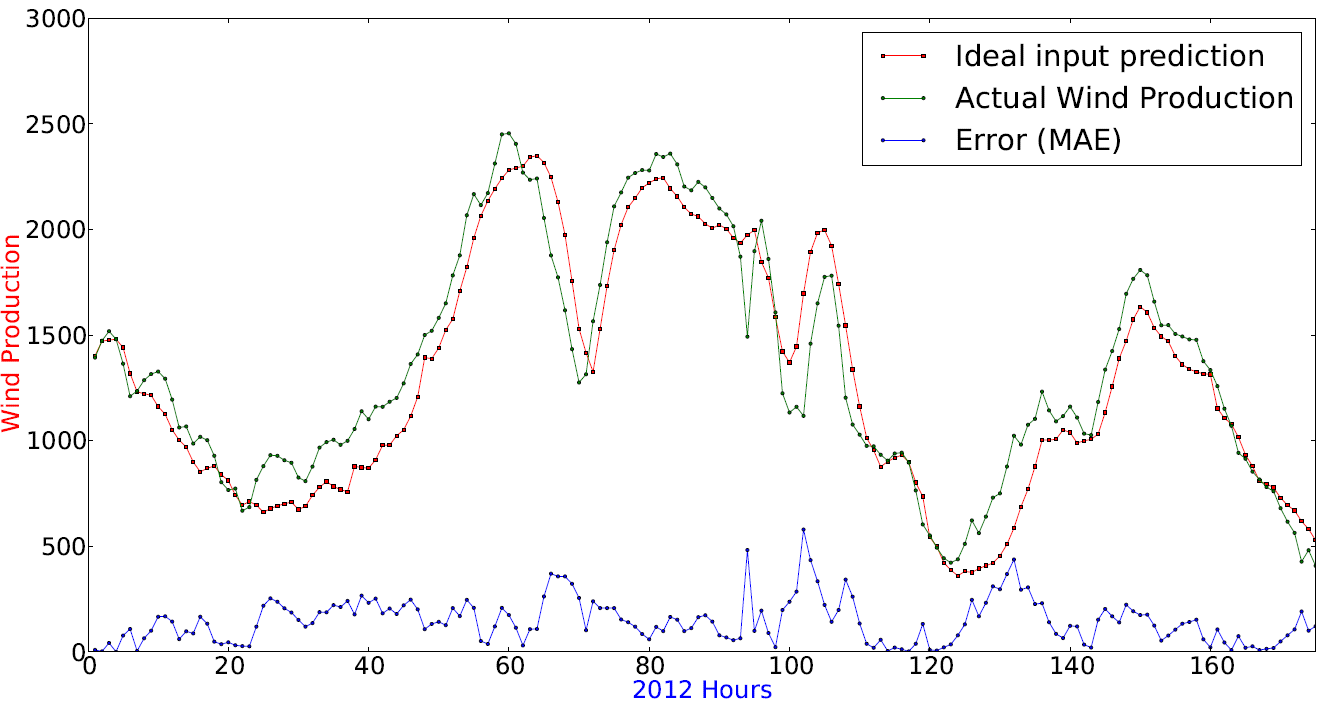
\includegraphics[width=0.99\linewidth]{billeder/bestInputParameterPrediction.png}
\caption{Wind production prediction for 0-175 hours in 2012 with the best combination}
\label{fig:bestInputParameterPrediction}
\end{figure} 

\begin{figure}[H]
\centering
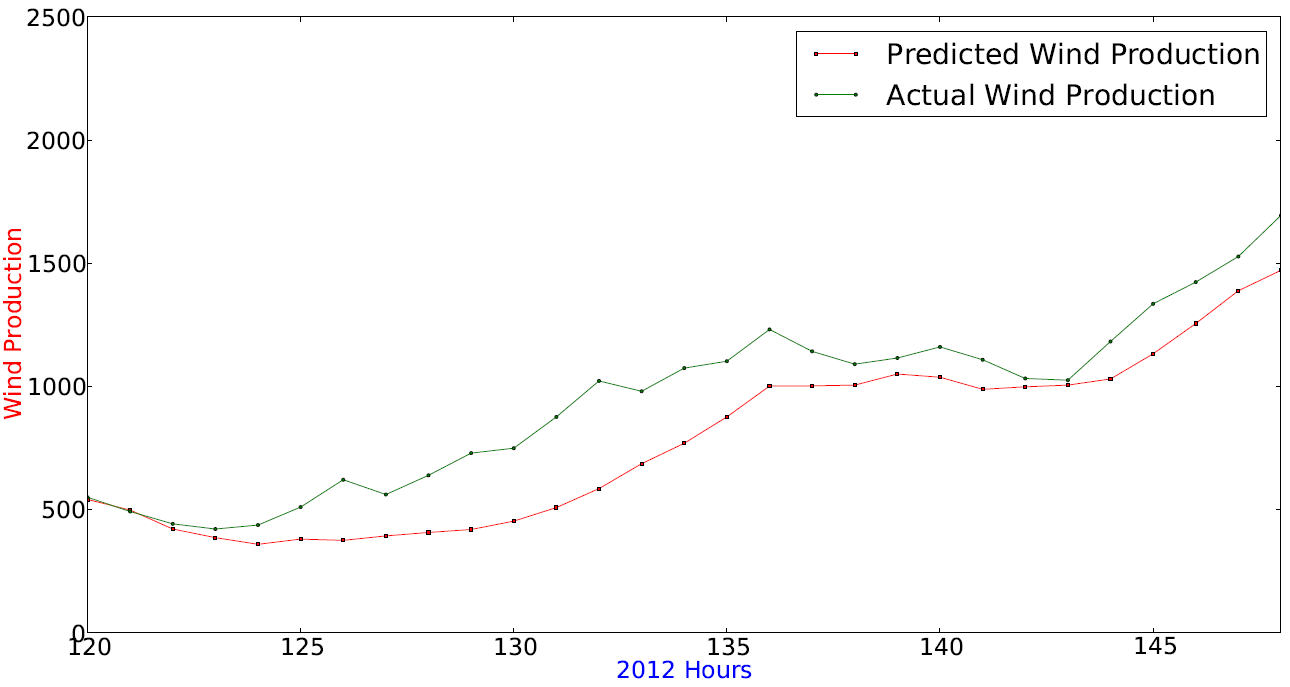
\includegraphics[width=0.99\linewidth]{billeder/bestInputCombi120-148.png}
\caption{Wind production prediction for 24 hours between 120 and 148}
\label{fig:bestInputCombi120-148}
\end{figure} 

\begin{figure}[H]
\centering
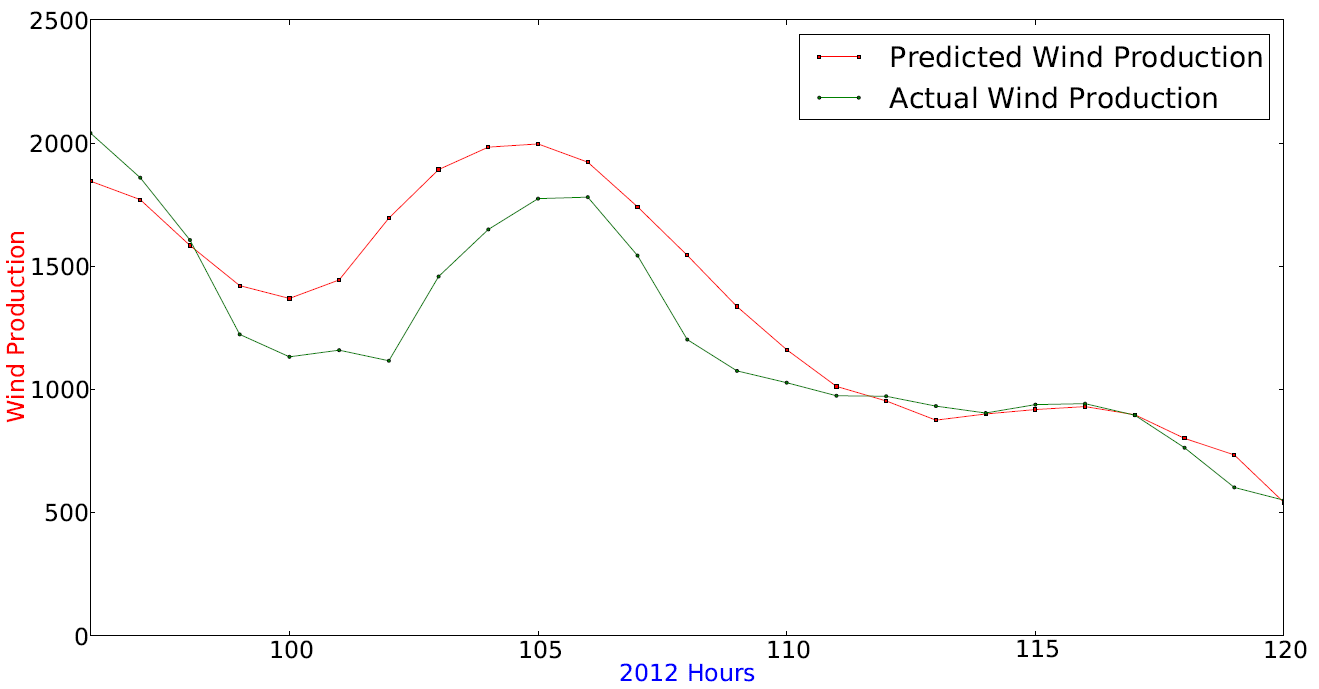
\includegraphics[width=0.99\linewidth]{billeder/bestInputCombi96-120.png}
\caption{Wind production prediction for 24 hours between 96 and 120}
\label{fig:bestInputCombi96-120}
\end{figure}   

\begin{figure}[H]
\centering
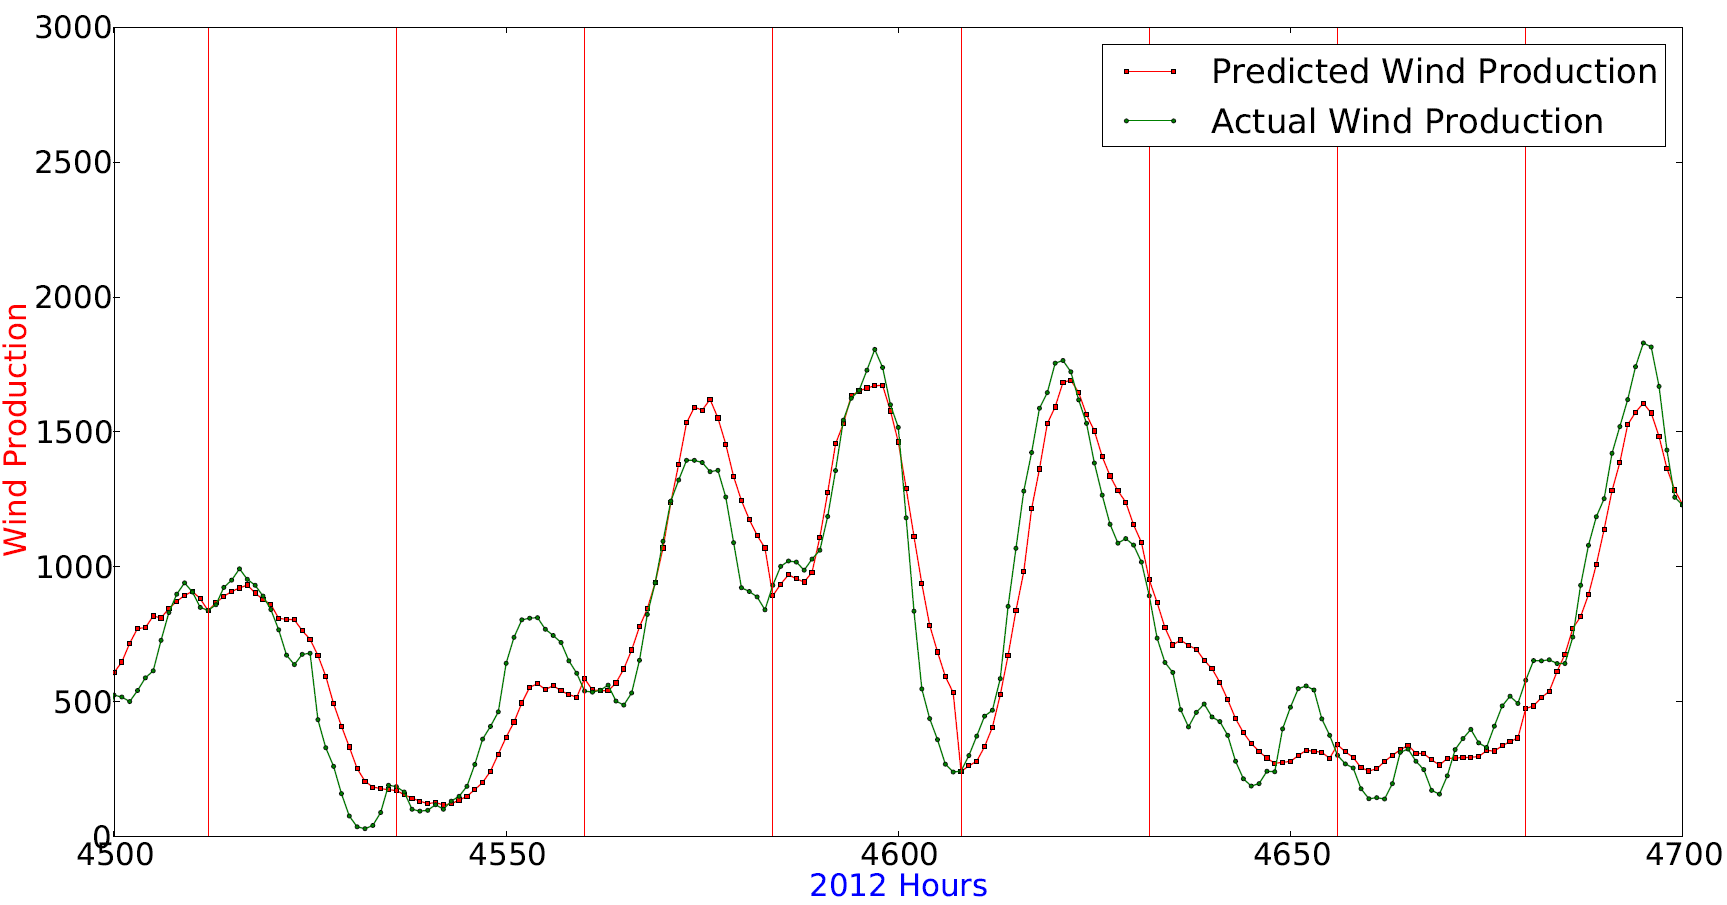
\includegraphics[width=0.99\linewidth]{billeder/bestInputCombi4500-4700.png}
\caption{Wind production prediction for 4500-4700 hours in 2012 with the best combination}
\label{fig:bestInputCombi4500-4700}
\end{figure} 

\begin{figure}[H]
\centering
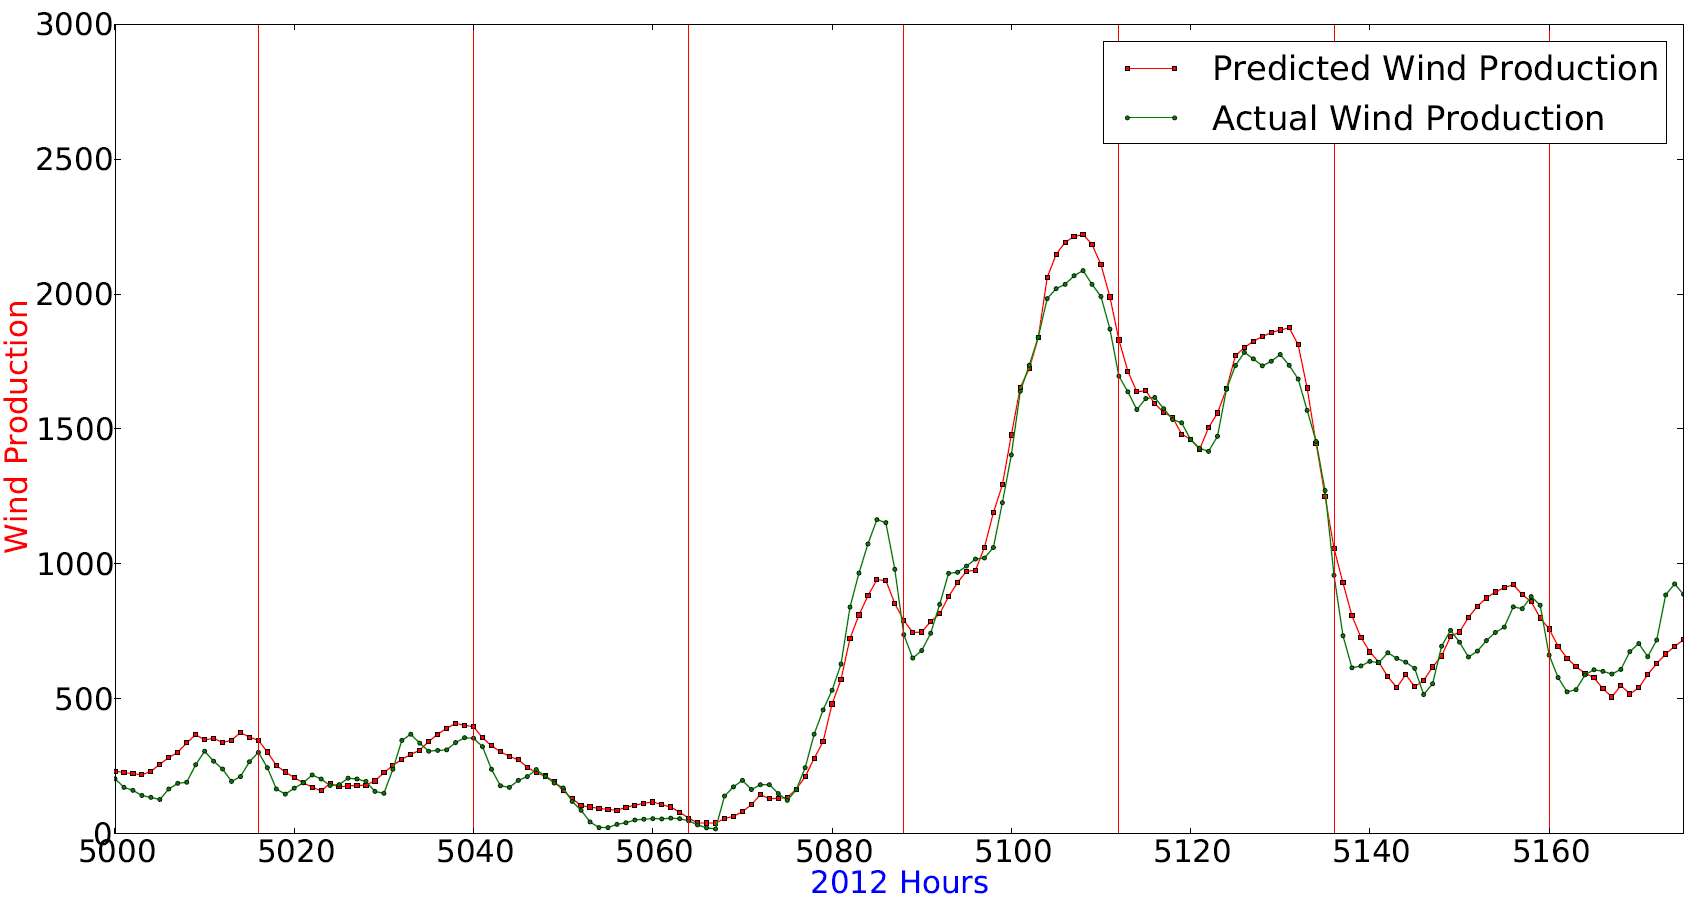
\includegraphics[width=0.99\linewidth]{billeder/bestInputParameterLowNumbers.png}
\caption{Wind production prediction for 5000-5175 hours in 2012 with the best combination}
\label{fig:bestInputParameterLowNumbers}
\end{figure}   

\subsubsection{Conclusion}
All results of the first experiment can be seen in Appendix~\ref{sec:windResultsAppendix}. The best result can be seen in Table~\ref{table:windProdInputParamsTop10}. The following conclusions can be made: 

\begin{enumerate}
\item Wind speed showed as expected to have very high significance when predicting the wind power production. Consumption was not represented in top-3 even though it showed very good co-relation in the analysis. The good relationship between temperature and consumption is described in Section~\ref{sec:consumptionWindProduction} which can explain why consumption in top 3 is omitted and substituted with either air density or temperature. The analysis in Section~\ref{sec:airDensity} describes how air density is calculated with temperature as the most significant factor since pressure is close to constant in the dataset.   
\item Last known production is highly represented in both top-10 and bottom-10. It is important when put together with the right combination but whenever in combination with month of year it worsens. Month did not help the prediction even though the dataset was increased to better incorporate the seasonality aspect. Air density and time of day both showed to be highly represented in top-10 and on both on top 3 together with wind speed and last known production.
\item Wind direction was expected little influence bot showed itself four times in top-10. It is assumed that direction is of some importance but not much based on the exact same constitution of input parameters just without wind direction achieved close to same result.
\end{enumerate}

The experiments to come will be based on input combinations from the top 3 from Table~\ref{table:windProdInputParamsTop10}. The inputs are:
\begin{itemize}
\item Wind speed;
\item Air density;
\item Wind Direction;
\item Temperature;
\item Last known production;
\item Time of day;
\end{itemize}
\newpage
\subsection{Experiment Two - Data Manipulation}
\label{sec:windProdExperimentTwo}
Experiment two tries to discover the best way to represent the input data. The need for manipulating the data can arise if irregularities exist that cannot be predicted or simply to adjust the data to better fit the inner workings of the neural network. The 3 approaches to data manipulation tested in the thesis is normalization, trimming and using a matrix as input. The necessity is described in more detail in Section~\ref{sec:DataManipulation}. Normalization is necessary for all input and is used in all experiments because the tanh function is used as activation function. Trimming is used to trim away irregularities if such exist but it does not apply for when predicting wind power production (see Section~\ref{sec:windProductionDev}). It does not leave out the possibility of scenarios where trimming makes sense when used in the hand of an expert, e.g. if experience can eliminate certain high values in the next 24 hours then they could be trimmed. We will investigate whether or not trimming makes the predicted values more accurate in relation to the same values in the predictions without trimming. Tests have been conducted to show the possible benefits from using trimming on wind power production --- both with a trimmed and untrimmed testing set. The purpose of experiment two is to turn inputs into a matrix whenever it makes sense and see the possible benefit of trimming. As described in Section~\ref{sec:Matrix} one input parameter is split into a input parameter for all of its possible values. Each value then has a weight that is adjusted according to the error as illustrated in Section~\ref{sec:annSection}. This is of course only an option if all values are known in advance and of a manageable size. When considering wind production forecasting this is valid for hours of the day, month and wind speed. Only wind speed and time of day will be tested here due to the omitting of the month parameter in experiment one. 

\subsubsection{Hypothesis} 
The matrix manipulation can be applied when values are of a manageable size as discussed in Section~\ref{sec:Matrix}. Based on those discussions the following is expected: 

\begin{enumerate}
\item According to the discussions matrix makes the most sense when values are equally distributed. This apply for time of day and therefore it is expected to see an improvement when matrix is applied here
\item Values are not equally distributed for wind speed and the expectation is instead a worsening in the prediction when applying matrix here.
\end{enumerate}

\subsubsection{Variables}
The variables used in this experiment series:

\begin{itemize}
\item Wind speed (WS).
\item Air density (AD).
\item Time of day (ToD).
\item Time of day as matrix indicated by (m).
\item Temperature (T).
\item Wind direction (WD).
\item Last known production (L-P).
\end{itemize}

\subsubsection{Prediction - Applying matrix}
The decrease in accuracy when using wind speed as a matrix can be seen in Table~\ref{table:theWindProdInputParamsTop10WithMatrix}. None of the best results contain wind speed as matrix and they only differ 3,02\% from the top result whereas the results with wind speed as matrix lies between 7,49\% and 23,14\%. The best result is the same as in Table~\ref{table:windProdInputParamsTop10} but number \#2 and \#3 has switched places but the difference between them is still not significant. All in top-3 improved with an average improvement of 1,9\%. The significance of time of day is seen in Section~\ref{sec:greenTOD} and the improvement was expected to be somewhat higher since the matrix should make it more expressive. Figure~\ref{fig:hourly_wind_production} shows a difference in average production from 750 during the night to around 925 during the day. The difference between the minimum production hour and the maximum is 16,2\% which might allow the one input parameter to generalize almost as good as the matrix implementation. Also the these numbers are for the entire year and since the training set in this case is only 3 month the difference between min and max will be even lower. If the difference in production between the hours of the day were bigger, lets say 900, the one parameter would still have to reflect the maximum and minimum in the same weight. This would be a problem if the majority were high and trying to predict a production represented in the minimum hour. The matrix implementation would instead consider each value by itself and have no impact on one another and is therefore expected to perform better. This scenario is illustrated in the analysis of price in Section~\ref{sec:seasonality} where Figure~\ref{fig:price_over_weekdays} shows a 42,4\% difference between the minimum price hour to the maximum price hour. The expectation is to see a better improvement when applying matrix to price because if this. 

Wind speeds are represented by 41 different values in our data set which can explain the decrease in accuracy. Instead of having only one input to represent each of the values, the matrix turned into 41 inputs for every single value. The purpose is to have a weight that tells exactly how much the specific wind speed in general influence the wind production to predict. The network will do so by adjusting a weight for the different wind speeds in the matrix whenever they are seen. As described in Section~\ref{sec:Matrix} a problem arise if some values does not exist or are under-represented. This will cause that specific value to be under-expressed because the weight has only been adjusted a few times or not at all. The seasonal differences in wind power production is described in Section~\ref{sec:windProdSeasonality} and since wind production follows wind speed the training set of only 3 months does not cover all wind speeds. Many wind speed will therefore be under-represented when using wind speed as matrix. This is also backed up by the results.

\begin{center}
\begin{longtable}{|c|c|c|c|c|c|c|c|c|c|c|c|}
\hline
\textbf{WS} & \textbf{AD} & \textbf{C} & \textbf{T} & \textbf{WD} & \textbf{L-P} & \textbf{ToD} & \textbf{MAE} & \textbf{\% from \#1} &  \textbf{H1} & \textbf{H2} & \textbf{\% CD}   \\
\hline
\endfirsthead
\multicolumn{12}{c}%
{\tablename\ \thetable\ -- \textit{Continued from previous page}} \\
\hline
\textbf{WS} & \textbf{AD} & \textbf{C} & \textbf{T} & \textbf{WD} & \textbf{L-P} & \textbf{ToD} & \textbf{MAE} & \textbf{\% from \#1} &  \textbf{H1} & \textbf{H2} & \textbf{\% CD}  \\
\hline
\endhead
\hline \multicolumn{12}{r}{\textit{Continued on next page}} \\
\endfoot
\hline
\endlastfoot
\arrayrulecolor{light-gray}
 \x &  &  &  \x &  &  \x &  \x (m) & 126,25 & 0,0\% & 18 & 17 & 71\% \\ \hline
 \x &  \x &  &  &  &  \x &  \x (m) & 127,95 & 1,35\% & 13 & 19 & 70\% \\ \hline
 \x &  \x &  &  &  \x &  \x & \x (m) & 130,07 & 3,02\% & 2 & 23 & 69\% \\ \hline
 \x (m) & &  &  \x &  &  \x &  \x (m) & 135,71 & 7,49\% & 13 & 16 & 67\% \\ \hline
 \x (m) & \x &  &  &  \x &  \x &  \x & 144,44 & 14,41\% & 14 & 12 & 70\% \\ \hline
  \x (m) & \x &  &  &  &  \x &  \x & 147,63 & 17,12\% & 8 & 16 & 70\%\\ \hline
 \x (m) & \x &  &  &  \x &  \x &  \x (m) & 149,18 & 18,16\% & 13 & 21 & 62\% \\ \hline
 \x (m) & &  &  \x &  &  \x &  \x & 149,19 & 18,17\% & 10 & 22 & 63\% \\ \hline
 \x (m) & \x &  &  &  &  \x &  \x (m) & 155,46 & 23,14\% & 16 & 13 & 59\% \\ \hline
\caption{Matrix test}
\label{table:theWindProdInputParamsTop10WithMatrix}
\end{longtable}
\end{center}

\begin{center}
\begin{longtable}{|c|c|}
\hline
\textbf{MAPE} & \textbf{MAE} \\
\hline
\endfirsthead
\multicolumn{2}{c}%
{\tablename\ \thetable\ -- \textit{Continued from previous page}} \\
\hline
\textbf{MAPE} & \textbf{MAE} \\
\hline
\endhead
\hline \multicolumn{2}{r}{\textit{Continued on next page}} \\
\endfoot
\hline
\endlastfoot
\arrayrulecolor{light-gray}
18,94\% & 126,25 \\ \hline
19,3\% & 127,95\\ \hline
19,52\% & 130,07 \\ \hline
20,36\% & 135,71\\ \hline
21,67\% & 144,44\\ \hline
22,15\% & 147,63 \\ \hline
22,38\% & 149,18\\ \hline
22,38\% & 149,19 \\ \hline
23,32\% & 155,46 \\ \hline
\caption{Average prediction MAE/MAPE on unseen data vs. prediction MAE/MAPE on training set with matrix}
\label{table:predictionMAEUnseenVsTrainingSetSeasonality}
\end{longtable}
\end{center}

\subsubsection{Prediction - Trimming}
The need for trimming exists if irregularities exist or you want to narrow the narrow down the dataset and focus the prediction. In wind power production such values do not exist in our dataset because we want to predict all values over the entire year. This does leave out the possibility that trimming could make the prediction more accurate on certain values outside of the trimmed values. This is disproved in the context of wind power in Table~\ref{table:trimmingOnBothSetsTable} where all types of trim results in a worsening in MAE. This indicates that values that are necessary for the generalization function to approach its target are removed during trimming. What can be seen though is that the more trim the better it becomes. Section~\ref{sec:windProductionDev} shows how the trimming would affect the dataset and it is clear that when values are removed it cuts directly in a curve. It results in the possibility of actually creating irregularities. This confirmed by comparing the graph in Figure~\ref{fig:fivePercentTrimPrediction} with the one in Figure~\ref{fig:bestInputPredictFrom0-400}. The curves are not as smooth which is obvious in most of the predicted hour but especially in 48-82 compared to the hours without trimming. It is not the exact same hours that are predicted but it shows how the graph is cut up and becomes more volatile and harder to predict.

\begin{center}
\begin{longtable}{|c|c|c|c|c|c|c|}
\hline
\textbf{Trim \%} & \textbf{MAPE}  & \textbf{MAE} & \textbf{\% Ranking} & \textbf{Min trim} & \textbf{Max trim} & \textbf{\% CD} \\
\hline
\endfirsthead
\multicolumn{7}{c}%
{\tablename\ \thetable\ -- \textit{Continued from previous page}} \\
\hline
\textbf{Trim \%} & \textbf{MAPE} & \textbf{MAE} & \textbf{\% Ranking} & \textbf{Min trim} & \textbf{Max trim} & \textbf{\% CD} \\
\hline
\endhead
\hline \multicolumn{7}{r}{\textit{Continued on next page}} \\
\endfoot
\hline
\endlastfoot
\arrayrulecolor{light-gray}
5\% & 19,21\% & 128,91 & 0,0\% & 40 & 2018 & 69\% \\ \hline  
4\% & 19,73\% &  130,94 & 1,57\% & 14 & 2076 & 73\% \\ \hline  
3\% & 20,5\% & 134,19 & 4,1\% & 49 & 2154 & 72\%\\ \hline 
2\% & 20,96\% & 136,27 & 5,71\% & 23 & 2270 & 72\% \\ \hline  
1\% & 20,92\% &  138,19 & 7,2\% & 31 & 2416 & 72\%\\ \hline 
\caption{Trimming from 1\% to 5\%}
\label{table:trimmingOnBothSetsTable}
\end{longtable}
\end{center}
\todo{make it}

\begin{figure}[H]
\centering
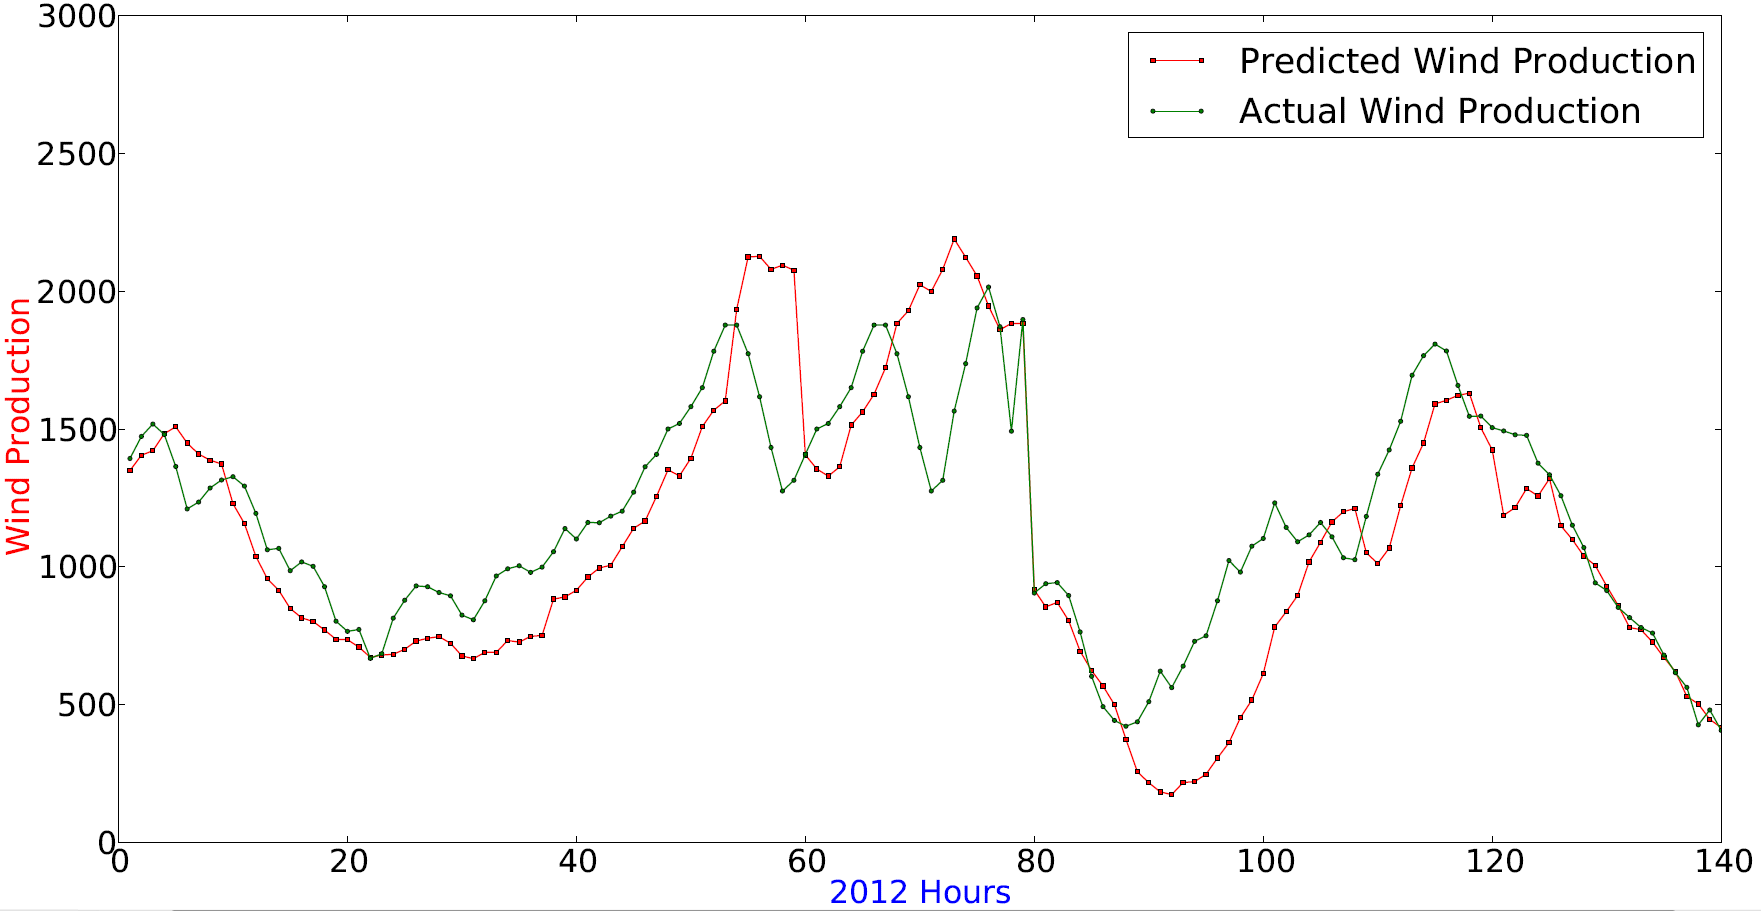
\includegraphics[width=0.99\linewidth]{billeder/fivePercentTrimPrediction.png}
\caption{Wind power prediction for hours 0-400 with 5\% trim}
\label{fig:fivePercentTrimPrediction}
\end{figure} 

\begin{figure}[H]
\centering
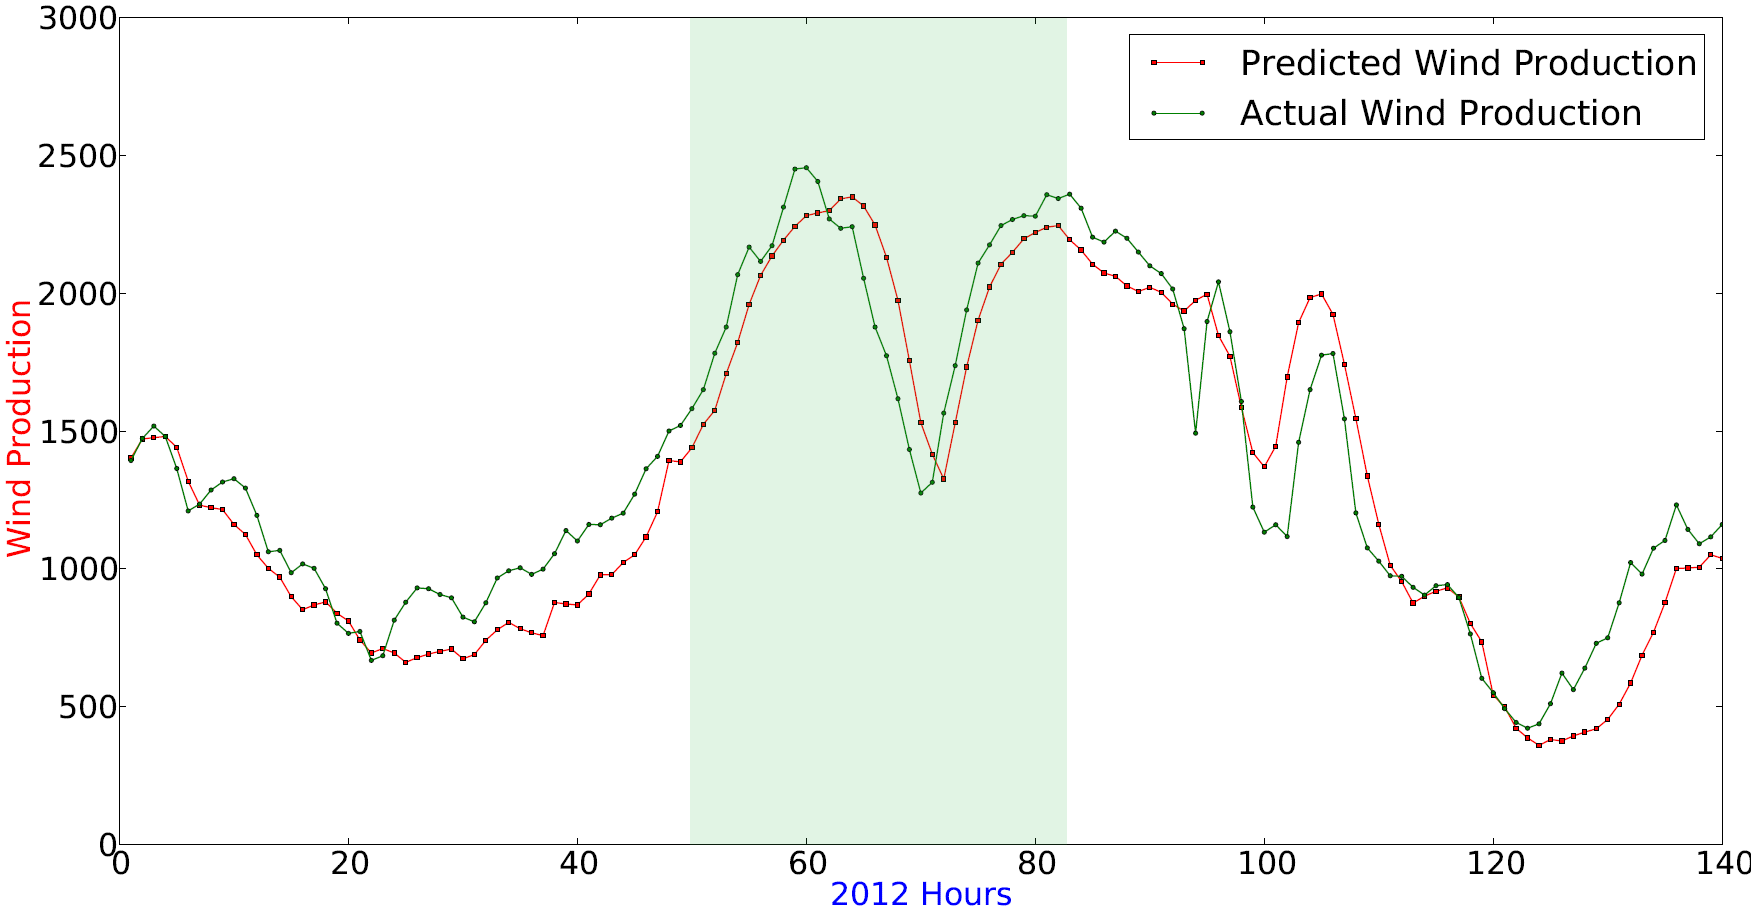
\includegraphics[width=0.99\linewidth]{billeder/bestInputPredictFrom0-400.png}
\caption{Wind power prediction for hours 0-400 with best input combination}
\label{fig:bestInputPredictFrom0-400}
\end{figure} 

\subsubsection{Best prediction graph}
The prediction in Figure~\ref{fig:bestMatrixGraph} is much similar to what was seen in the best prediction from experiment one which is also indicated by the small difference in error. See Section~\ref{sec:bestInputCombiGraph}. 

\begin{figure}[H]
\centering
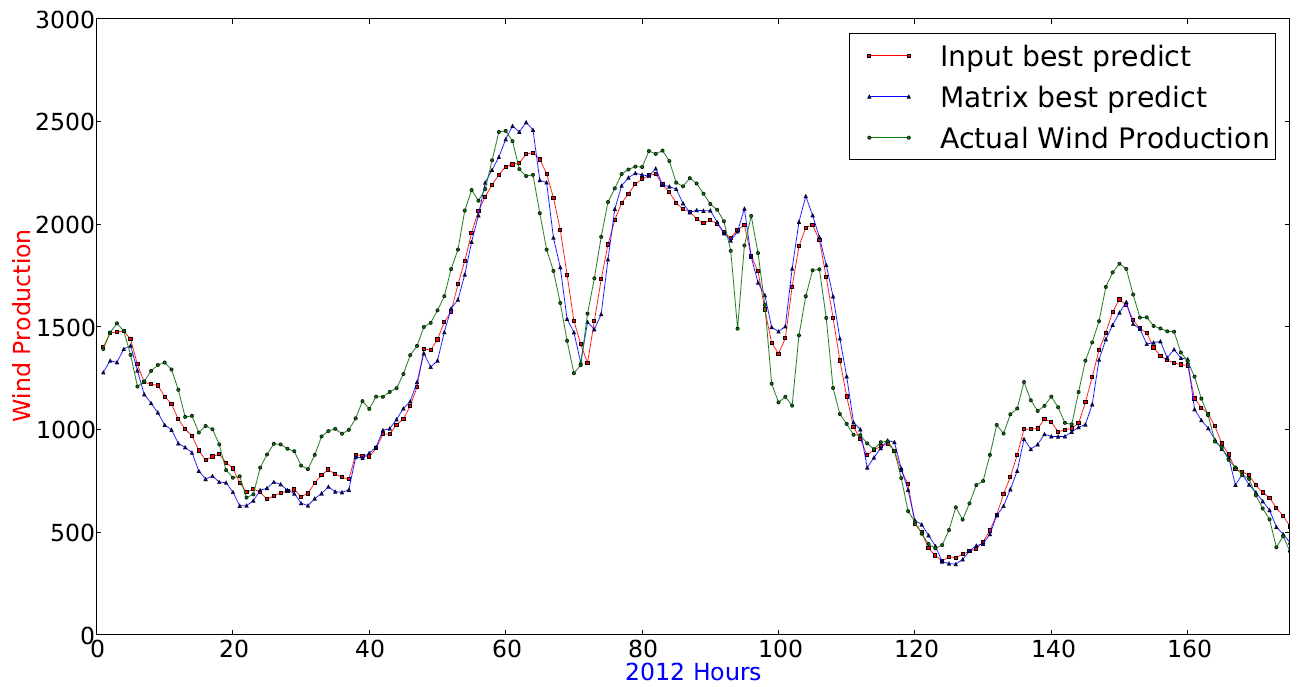
\includegraphics[width=0.99\linewidth]{billeder/bestMatrixGraph.png}
\caption{Wind power prediction for 175 hours in 2012 for the best matrix experiment}
\label{fig:bestMatrixGraph}
\end{figure}   

\subsubsection{Conclusion}
Matrix has been applied to time of day and wind speed. Experiments have been conducted to find where matrix is best applicable.

\begin{enumerate}
\item When applying matrix to time of day there is a slight improvement and it outperformed all predictions with wind speed as matrix. The time of day with matrix predictions are all better than their corresponding prediction in Table~\ref{table:windProdInputParamsTop10}. The improvement is in average only 1,9\% in MAE which is not as significant as expected and it can therefore be argued if matrix is worth the enlargement in input parameters when predicting wind power production. Trade-offs must be made in relation to the time to process and the achieved improvement. The trade-off between time and inputs will be discussed further in a later experiment 
\item The decrease in performance when applying matrix to wind speed can be seen from the results in Table~\ref{table:theWindProdInputParamsTop10WithMatrix}. The decrease can be due to the wind speed values not being equally distributed and therefore in some cases be under-represented and not able to be expressed properly.  
\end{enumerate}

The improvement by applying matrix to time of day is considered enough for next experiment under the circumstances of our test procedure from Section~\ref{sec:testProcedure}. Wind speed as matrix will be omitted.

\newpage

\subsection{Experiment Three - Calculated Inputs}
The experiments here will be focusing on the concepts described in Section~\ref{sec:usingStatisticalInput}. The importance of the current wind production development is described in Section~\ref{sec:windProductionDev} and it describes how the wind production has high volatility and follow certain tendencies. The purpose is to add inputs that in some way analyse productions from immediate past hours to help the existing generalization approach its target more accurately in a specific hour. We therefore see it as independent from the input analysis since it will help the best of the input combinations to perform better. All of the approaches take outset in previous hours so the first step is to find the best number of previous hours to calculate upon. Secondly, they must be tested in combination with each other to find the best combination. The different approaches are historical volatility, skewness, simple, slope calculation and inclusion of previous productions as input. 

\subsubsection{Hypothesis} 
It is the hypothesis that the different approaches will help the neural network approach its target better by adding knowledge about the current trend for every hour. It leads to: 

\begin{enumerate}
\item Wind production is volatile and therefore it is expected that the historical volatility will help the generalization to approach its target.
\item Section~\ref{sec:windProductionDev} explains the need for identifying the development of the curve. Beside from historical volatility it comes in 3 different approaches: 1) skewness; 2) slope calculation and 3) previous productions as input. The expectation is to see a slight increase in performance when these are applied.
\item It is the expectation to achieve better accuracy when combining the different approaches.
\end{enumerate}

\subsubsection{Variables}
The variables used in this experiment series:

\begin{itemize}
\item Wind speed (WS).
\item Air density (AD).
\item Time of day as matrix (ToD).
\item Temperature (T).
\item Wind direction (WD).
\item Last known production (L-P).
\item Historical volatility (V).
\item Skewness (S).
\item Simple slope calculation (C).
\item Previous productions as input (Scatter/Sc)
\end{itemize}

\subsubsection{Prediction - Historical Volatility}
\label{sec:predictionHistVol}
Historical Volatility is presented in Section~\ref{sec:usingStatisticalInput}. The purpose is to calculate the historical volatility for one hour based on a predefined number of previous hours, e.g. every hour in the training set will calculate the historical volatility from for instance 20 hours just before it (except from the 20 first hours). The volatility calculation will be based on EWMA from Section~\ref{sec:ewmaVolatility} which requires a smoothing factor between 0-1 that needs to be found through experiments. The experiment will be conducted for smoothing factors between 0,1 and 0,9 on hours between 4-24. When the best rate with the best number of hours has been established for the dataset it will be tested on top-3 from Table~\ref{table:theWindProdInputParamsTop10WithMatrix}. The improvement is 3,52\% better than the best prediction without it. 

\footnotesize
\begin{center}
\begin{longtable}{|c|c|c|c|c|c|}
\caption{Wind Production Input Parameter Test}\\
\hline
\textbf{Previous Hours} & \textbf{Smoothing factor}& \textbf{MAPE} & \textbf{MAE} & \textbf{\% Deviation} & \textbf{\% Correct Direction} \\
\hline
\endfirsthead
\multicolumn{6}{c}%
{\tablename\ \thetable\ -- \textit{Continued from previous page}} \\
\hline
\textbf{Previous Hours} & \textbf{Smoothing factor}& \textbf{MAPE} & \textbf{MAE} & \textbf{\% Deviation} & \textbf{\% Correct Direction} \\
\hline
\endhead
\hline \multicolumn{6}{r}{\textit{Continued on next page}} \\
\endfoot
\hline
\endlastfoot
\arrayrulecolor{light-gray}
6 & 0,70 & 18,28\% & 121,81 & 0,0\% & 73\% \\ \hline
20 & 0,80 & 18,44\% & 122,9 & 0,89\% & 70\%  \\ \hline
24 & 0,60 & 18,47\% & 123,13 & 1,08\% & 71\& \\ \hline
24 & 0,80 & 18,61\% & 124,02 & 1,81\% & 70\% \\ \hline
16 & 0,20 & 18,85\% & 125,65 & 3,15\% & 69\% \\ \hline
12 & 0,30 & 19,05\% & 127,0 & 4,26\% & 70\% \\ \hline
24 & 0,70 & 19,06\% & 127,06 & 4,31\% & 69\% \\ \hline
16 & 0,60 & 19,11\% & 127,38 & 4,57\% & 69\% \\ \hline
24 & 0,40 & 19,13\% & 127,51 & 4,68\% & 70\% \\ \hline
16 & 0,90 & 19,17\% & 127,77 & 4,89\% & 69\% \\ \hline
\end{longtable}
\label{table:historicalVoltalityHours}
\end{center}
\normalsize

All combinations of smoothing factor and previous hours can be seen in Appendix~\ref{sec:historicalVolatiltiyResultsAppendix} --- only top 10 is shown here. The results in Table~\ref{table:historicalVoltalityHours} show that a smoothing factor of 0,70 calculated on the 6 previous hours is the best choice. The expectation was to get a low smoothing factor due to the fluctuations in the wind power production as described in Section~\ref{sec:ewmaVolatility}. The reason for the higher factor can be explained with the number of previous hours being too small to reflect the many changes. We can see from the graph in Figure~\ref{fig:bestVolatilityVsMatrixGraph} that the curves are much similar to the curves without volatility which is expected since the volatility approach is an augmentation of the best prediction with matrix. A noticeable difference is that the volatility under-shoots its targets in the bottom of many curves compared to the matrix approach in both Figure~\ref{fig:bestVolatilityVsMatrixGraph} and~\ref{fig:bestVolatilityVsMatrixGraph350-525}. It moves more rapidly from top to bottom. Another thing worth mentioning from Figure~\ref{fig:bestVolatilityVsMatrixGraph350-525} is how the addition of historical volatility is capable of predicting all the way to the top in 415 and 480 compared to the standard matrix prediction indicated by the blue line. The under- and overshooting compared to the matrix only prediction is also verified in Figure~\ref{volatilityBest700-1000}.

\begin{figure}[H]
\centering
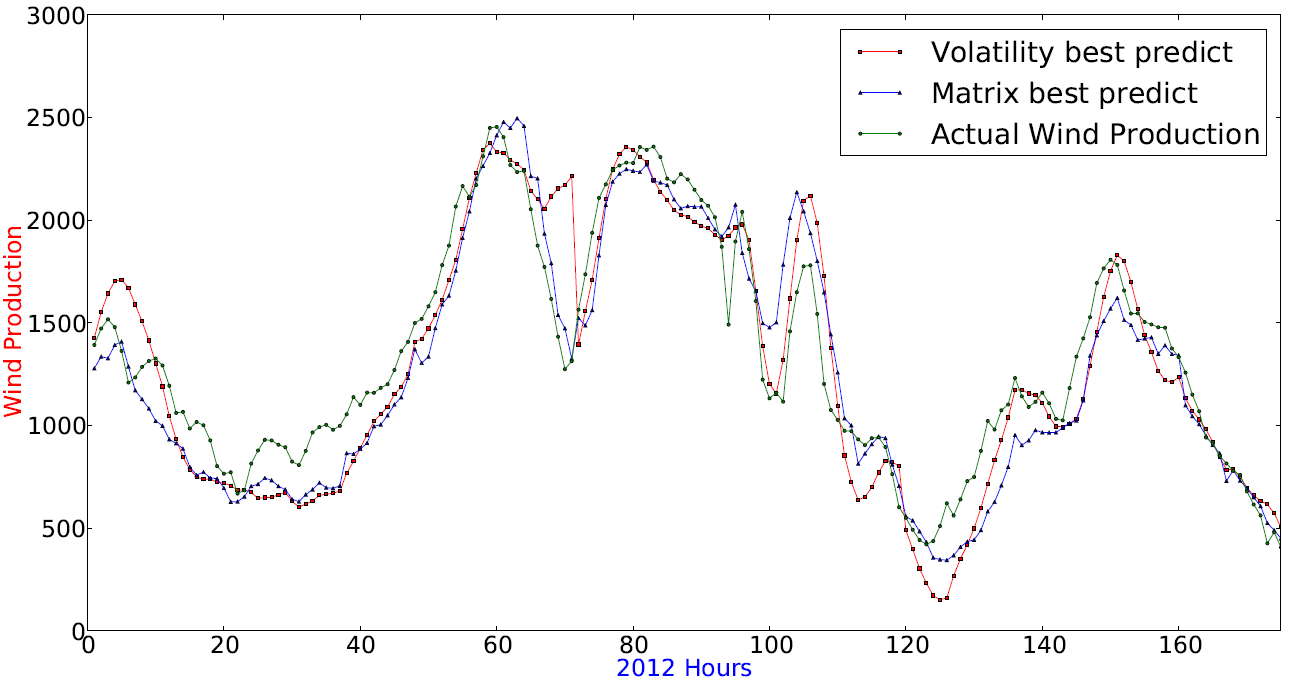
\includegraphics[width=0.99\linewidth]{billeder/bestVolatilityVsMatrixGraph.png}
\caption{Wind production prediction for hours 0-175 in 2012 with historical volatility as input}
\label{fig:bestVolatilityVsMatrixGraph}
\end{figure} 

\begin{figure}[H]
\centering
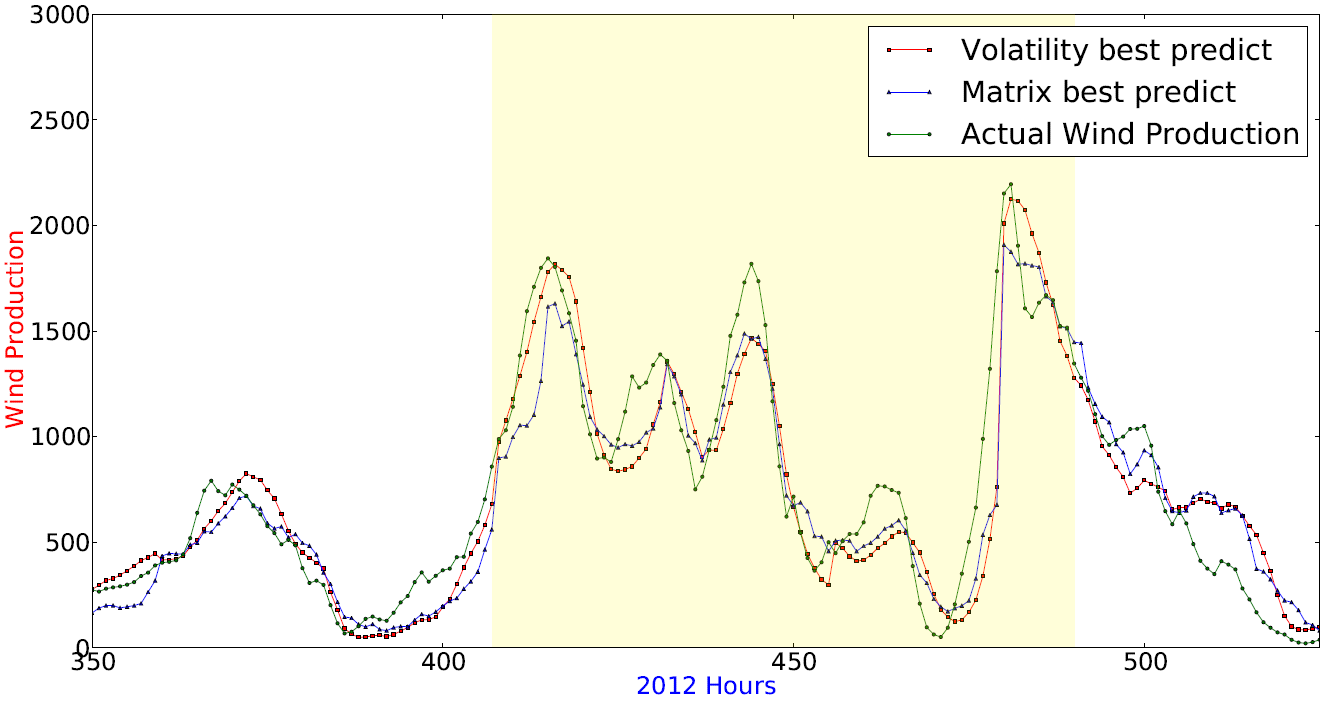
\includegraphics[width=0.99\linewidth]{billeder/bestVolatilityVsMatrixGraph350-525.png}
\caption{Wind production prediction for hours 350-525 hours in 2012 with historical volatility as input}
\label{fig:bestVolatilityVsMatrixGraph350-525}
\end{figure} 

\begin{figure}[H]
\centering
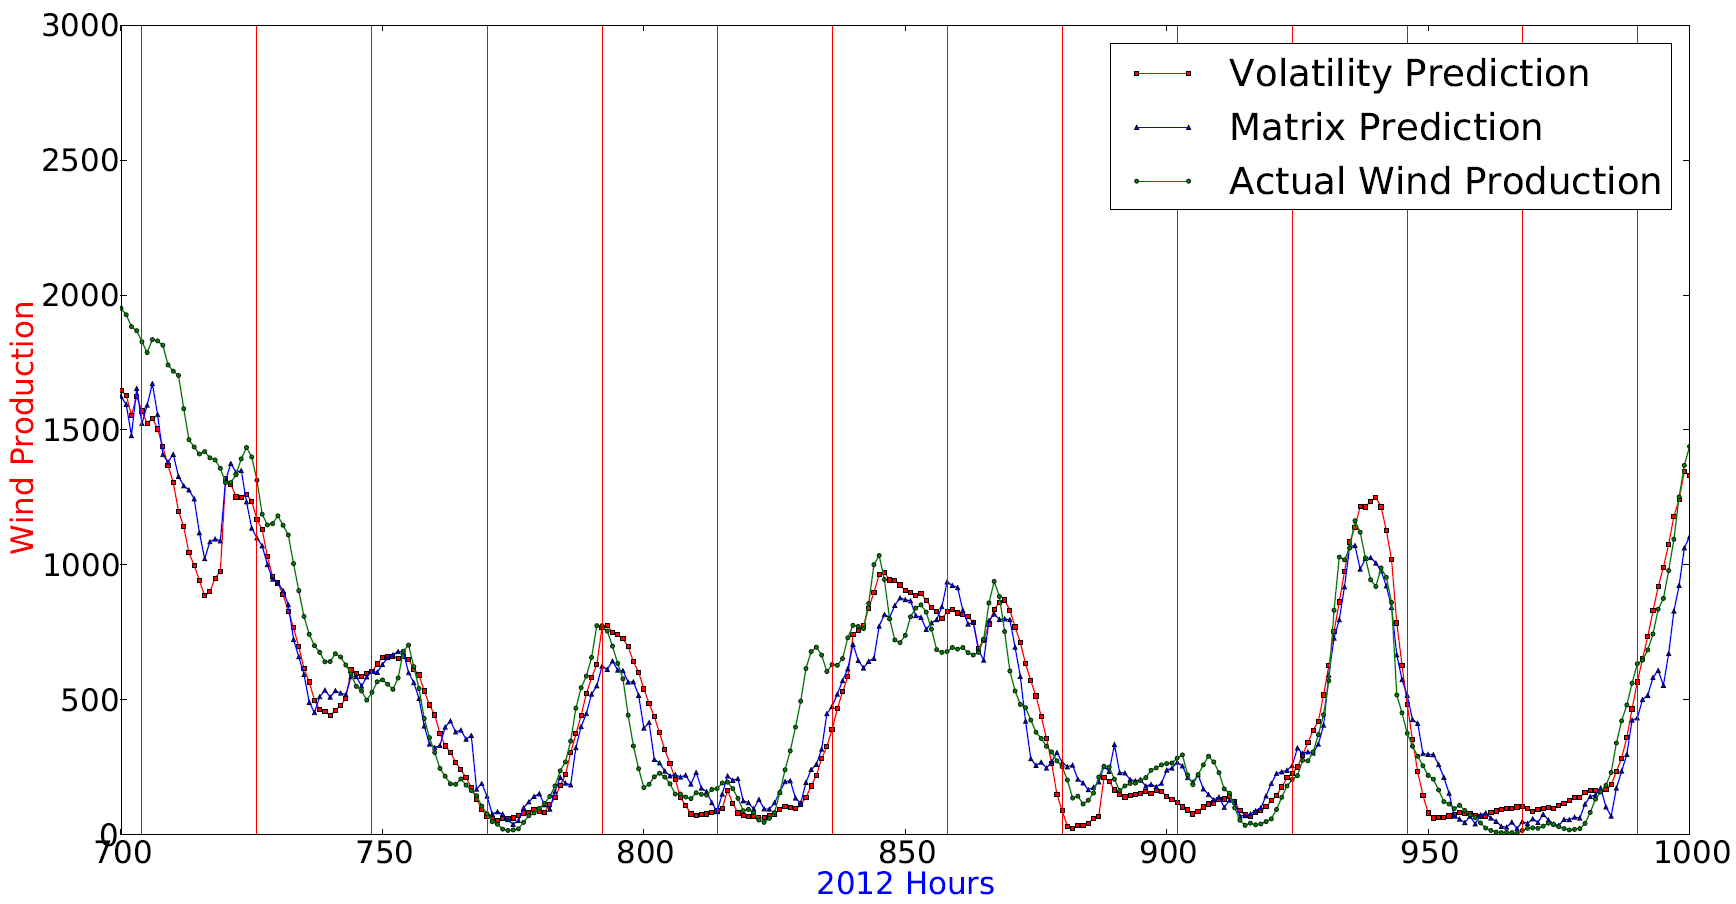
\includegraphics[width=0.99\linewidth]{billeder/volatilityBest700-1000.png}
\caption{Wind production prediction for hours 700-1000 hours in 2012 with historical volatility as input}
\label{fig:volatilityBest700-1000}
\end{figure} 

\subsubsection{Prediction - Skewness}
Skewness is a calculation of how much a distribution leans to one side of the mean which is described in more detail in Section~\ref{sec:skewness}. What is important to identify is again how many previous hours to include in the calculation of the skew in order to get the best picture of what side the curve is currently leaning towards. Table~\ref{table:skewnessHours} shows results where the best fit is found to be 16 hours. This will be basis for further testing when trying to use the methods in combination to see if any of them can augment each other. At first glance skewness does not seem to improve much but it will need testing when put together with the other calculations.

\begin{center}
\begin{longtable}{|c|c|c|c|}
\hline
\textbf{Hours} & \textbf{MAPE} & \textbf{MAE} & \textbf{\% Correct Direction}\\
\hline
\endfirsthead
\multicolumn{4}{c}%
{\tablename\ \thetable\ -- \textit{Continued from previous page}} \\
\hline
\textbf{Hours} & \textbf{MAPE} & \textbf{MAE} & \textbf{\% Correct Direction}\\
\hline
\endhead
\hline \multicolumn{4}{r}{\textit{Continued on next page}} \\
\endfoot
\hline
\endlastfoot
\arrayrulecolor{light-gray}
16 & 18,88\% & 125,85 & 69\% \\ \hline
4 & 19,13\% & 127,52 & 70\% \\ \hline
24 & 19,45\% & 129,63 & 69\% \\ \hline
8 & 19,68\% & 131,18 & 68\% \\ \hline
12 & 19,69\% & 131,26 & 68\% \\ \hline
6 & 19,73\% & 131,51 & 68\% \\ \hline
20 & 20,23\% & 134,81 & 67\% \\ \hline
2 & 20,9\% & 139,33 & 66\% \\ \hline
\caption{Prediction With Skewness and different hours}
\label{table:skewnessHours}
\end{longtable}
\end{center}

Figure~\ref{fig:bestSkewnessGraph} shows the first 175 hours when using skewness as input compared to standard matrix when predicting. The matrix with skewness is much similar to the one without and will not be discussed in further detail. 

\begin{figure}[H]
\centering
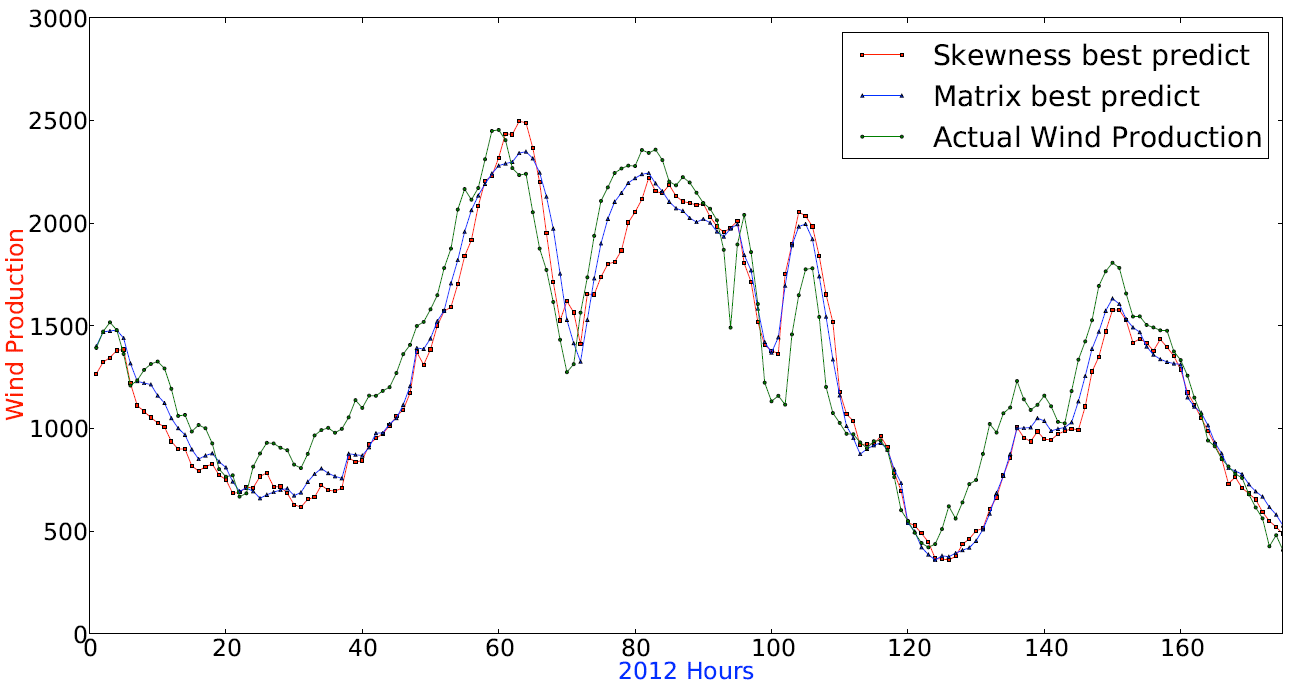
\includegraphics[width=0.99\linewidth]{billeder/bestSkewnessGraph.png}
\caption{Wind production prediction for 175 hours in 2012 with skewness as input}
\label{fig:bestSkewnessGraph}
\end{figure}    

\subsubsection{Prediction - Slope calculation}
\label{sec:windPowerSlopeCalc}
The experiment covers basic slope calculation of the curve. The intention is to get a notion of how much the previous productions have been going upwards before a particular hour. It captures how the slopes in general relate to the wind power production --- does a very steep slope in general affect the production to go up or not? Table~\ref{table:curveAnalysisHours} shows that the slope calculation as input does not work as intended. Its impact on the first 175 hours can be seen in Figure~\ref{fig:basicCurveAnalysisGrapho}. The best result from Table~\ref{table:curveAnalysisHours} calculates the slope from the previous 20 hours and the hours from 48-70 illustrates in the graph that it has a hard time identifying when to stop moving up since it has been moving up for so long. The 24-ahead prediction starts at 48 just before the drop and since the slope calculation is based on the last 20 hours it does not identify the shift --- it has a steep slope and points the overall generalization upwards since steep slopes in most cases result in ascending curves except when at the very top of one. The opposite happens around hour 70-80 where it does not know when to stop. This is a difference from the matrix without calculated inputs which is indicated by the blue line --- the prediction only follows the meteorological factors and how they relate to the production. The 1-hour-ahead forecasting with curve has been performed and obtains a MAE of 56,6. The graph can be seen in Figure~\ref{fig:curveOneAheadvs24Ahead} where the curve fitting as expected is significantly better.

\begin{center}
\begin{longtable}{|c|c|c|c|c|}
\hline
\textbf{Hours} & \textbf{MAPE} & \textbf{MAE} & \textbf{\% Correct Direction} \\
\hline
\endfirsthead
\multicolumn{4}{c}%
{\tablename\ \thetable\ -- \textit{Continued from previous page}} \\
\hline
\textbf{Hours} & \textbf{MAPE} & \textbf{MAE} & \textbf{\% Correct Direction} \\
\hline
\endhead
\hline \multicolumn{4}{r}{\textit{Continued on next page}} \\
\endfoot
\hline
\endlastfoot
\arrayrulecolor{light-gray}
20 & 20,0\% & 133,27 & 68\% \\ \hline
16 & 20,03\% & 133,52 & 67\% \\ \hline
12 & 20,56\% & 137,05 & 67\% \\ \hline
8 & 21,01\% & 140,0 & 70\% \\ \hline
24 & 21,98\% & 146,5 & 66\% \\ \hline
6 & 22,28\% & 148,5 & 67\% \\ \hline
2 & 22,75\% & 151,62 & 67\% \\ \hline
4 & 24,17\% & 161,12 & 66\% \\ \hline
\caption{Results for slope calculation as input on different previous hours}
\label{table:curveAnalysisHours}
\end{longtable}
\end{center}

\begin{figure}[H]
\centering
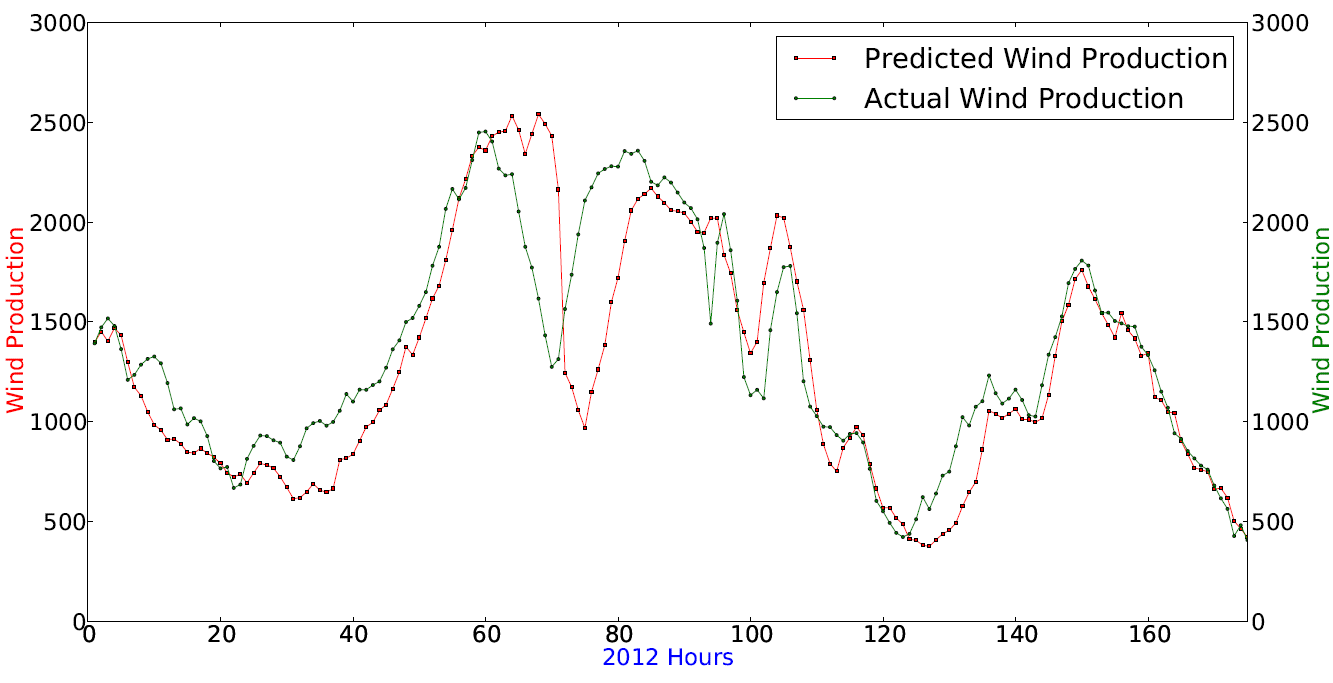
\includegraphics[width=0.99\linewidth]{billeder/curveAnalysisWindProduction.png}
\caption{Wind production prediction for 175 hours in 2012 with slope as input}
\label{fig:basicCurveAnalysisGrapho}
\end{figure} 

\begin{figure}[H]
\centering
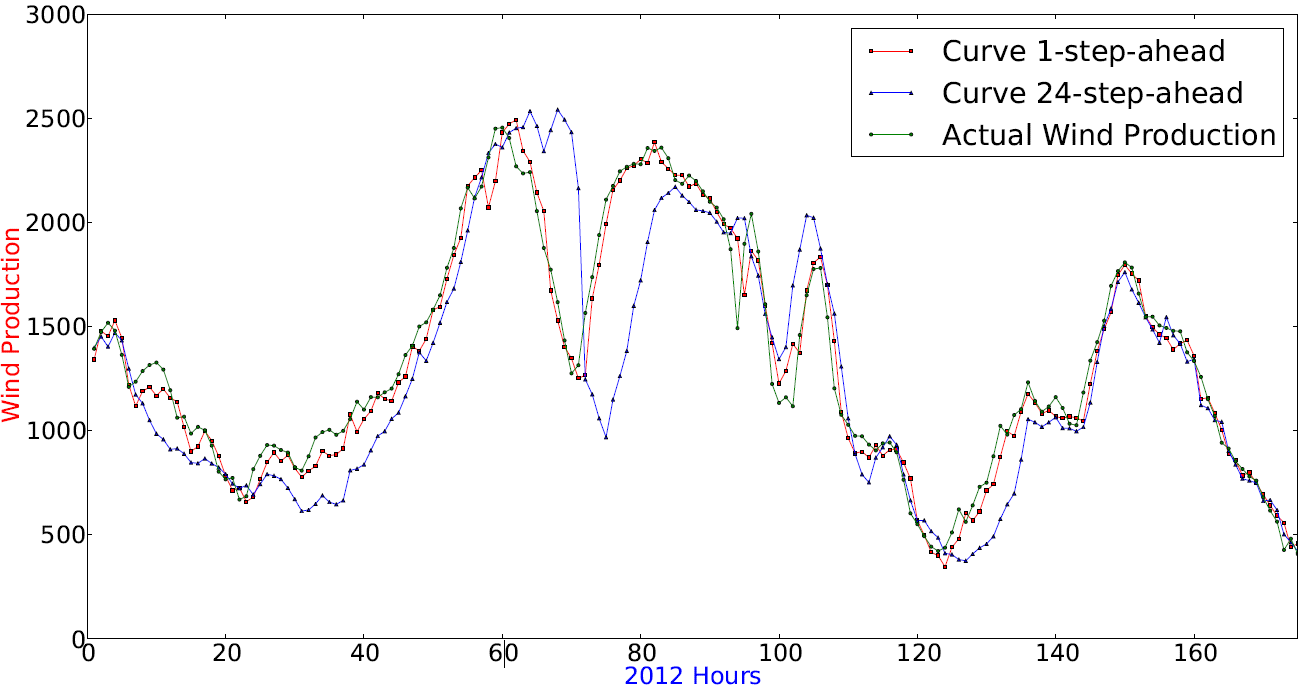
\includegraphics[width=0.99\linewidth]{billeder/curveOneAheadvs24Ahead.png}
\caption{1-step vs. 24-step ahead wind power predictions with curve}
\label{fig:curveOneAheadvs24Ahead}
\end{figure}   

\subsubsection{Combining the approaches}
\label{sec:combiningTheApproachesWP}
Experiments with combinations of the approaches have been performed to investigate whether or not any of them augment each other. Furthermore, adding historical productions as input has been tried as presented in Section~\ref{sec:scatterPaper} and discussed in Section~\ref{sec:scatterStrategy}. The approach adds 3 inputs for the production from one day ago, 3 inputs from the production one week ago, one input from the production two weeks ago, one input from the production three weeks ago and one last input from four weeks ago. The purpose is letting the network itself capture the price development over time instead of calculating it beforehand. Experiment results from each approach is in Table~\ref{table:comparisonStatistics} where the historical volatility with a smoothing factor of 0,70 and 6 previous hours outperforms the other approaches. 

\begin{center}
\begin{longtable}{|c|c|c|c|}
\hline
\textbf{Type} & & \textbf{MAPE} \textbf{MAE} & \textbf{\% Correct Direction} \\
\hline
\endfirsthead
\multicolumn{4}{c}%
{\tablename\ \thetable\ -- \textit{Continued from previous page}} \\
\hline
\textbf{Type} & & \textbf{MAPE} \textbf{MAE} & \textbf{\% Correct Direction} \\
\hline
\endhead
\hline \multicolumn{4}{r}{\textit{Continued on next page}} \\
\endfoot
\hline
\endlastfoot
\arrayrulecolor{light-gray}
Volatility, 0,70 as smoothing on 6 hours & 18,28\% & 121,81 & 73\% \\ \hline
Skewness with 16 hours & 18,88\% & 125,85 & 69\% \\ \hline
Scatter of prices & 20.0\% & 134,7 & 68\% \\ \hline
Slope as input with 20 hours & 20,0\% & 133,27 & 68\% \\ \hline
\caption{Comparison of the approaches}
\label{table:comparisonStatistics}
\end{longtable}
\end{center}

Skewness and curve in combination with each other achieves the best result but does not improve the results from Table~\ref{table:theWindProdInputParamsTop10WithMatrix}. The problem is most likely that the analysis of the curve gets to high priority in the generalization when trying to predict 24-ahead. When trying to predict a scenario totally different from what has just been seen, the calculated inputs will pull the generalization in the direction of the previous which we can see from Figure~\ref{fig:bestStatisticalApproachGraph}. Without the calculated inputs the generalization relies heavily on wind speed which was established in the analysis in Section~\ref{sec:windPowerAnalysis} but this will be contradicted by the calculated inputs that believe the curve to be heading in another direction because we are at the edge. The prediction relies heavily on where to predict from. The best of the calculated approaches based on the above results are volatility as only input with a MAE of 121,81.

\begin{figure}[H]
\centering
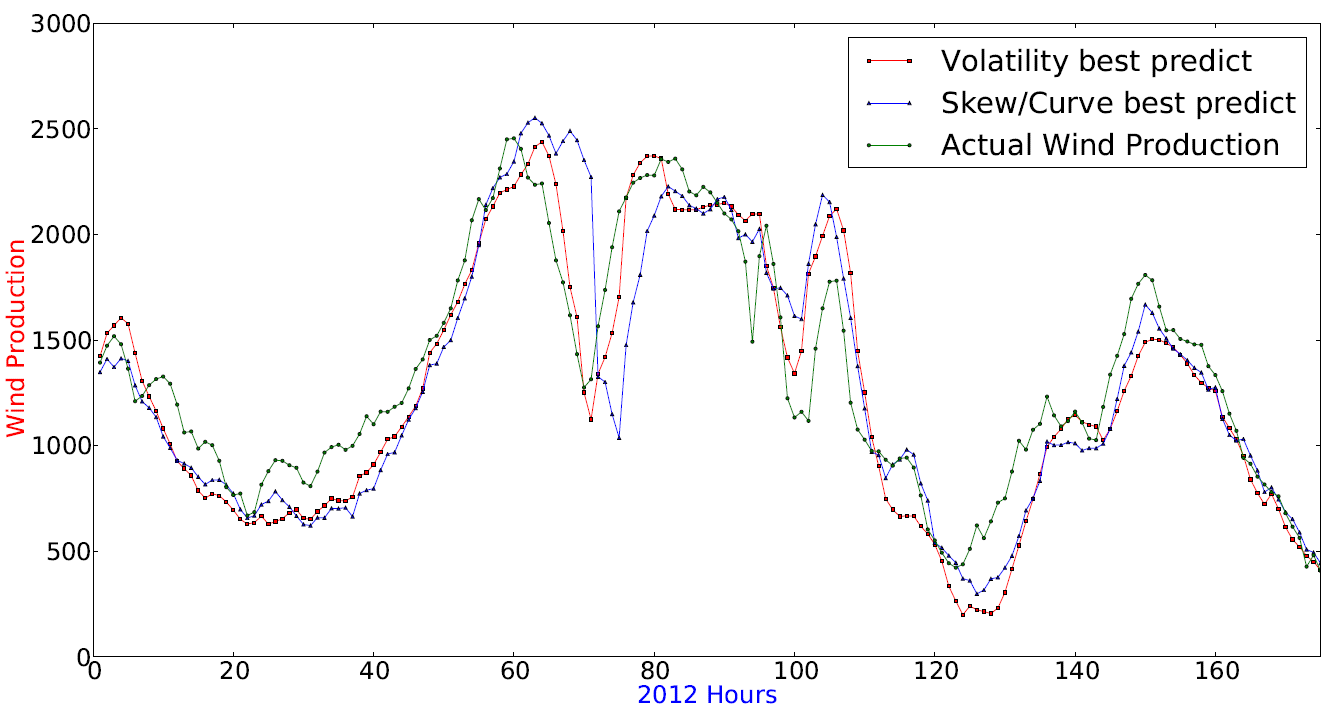
\includegraphics[width=0.99\linewidth]{billeder/bestStatisticalApproachGraph.png}
\caption{Wind production prediction for hours 120-144 in 2012 with historical volatility}
\label{fig:bestStatisticalApproachGraph}
\end{figure} 

\begin{center}
\begin{longtable}{|c|c|c|c|c|c|c|c|}
\hline
\textbf{Vola} & \textbf{Skew} & \textbf{Scat} & \textbf{Curve} & \textbf{MAPE} & \textbf{MAE} & \textbf{\% Rank} & \textbf{\% Correct Direction} \\
\hline
\endfirsthead
\multicolumn{8}{c}%
{\tablename\ \thetable\ -- \textit{Continued from previous page}} \\
\hline
\textbf{Vola} & \textbf{Skew} & \textbf{Scat} & \textbf{Curve} & \textbf{MAPE} & \textbf{MAE} & \textbf{\% Rank} & \textbf{\% Correct Direction} \\
\hline
\endhead
\hline \multicolumn{8}{r}{\textit{Continued on next page}} \\
\endfoot
\hline
\endlastfoot
\arrayrulecolor{light-gray}
 &  \x &  &  \x & 19,76\% & 131,69 & 0,0\% & 69\% \\ \hline
 \x &  \x &  &  & 20,96\% & 139,73 & 6,11\% & 72\% \\ \hline
 \x &  \x &  \x &  & 21,65\% & 144,33 & 9,6\% & 72\% \\ \hline
 \x &  \x &  &  \x & 22,35\% & 148,94 & 13,1\% & 72\% \\ \hline
 \x &  &  \x &  & 22,4\% & 149,31 & 13,38\% & 71\% \\ \hline
 \x &  &  &  \x & 22,93\% & 152,85 & 16,07\% & 71\% \\ \hline
 &  \x &  \x &  & 23,37\% & 155,74 & 18,26\% & 72\% \\ \hline
 &  &  \x &  \x & 23,44\% & 156,25 & 18,65\% & 72\% \\ \hline
 &  \x &  \x &  \x & 23,66\% & 157,69 & 19,74\% & 72\% \\ \hline
 \x &  \x &  \x &  \x & 25,74\% & 171,54 & 30,26\% & 71\% \\ \hline
 \x &  &  \x &  \x & 26,06\% & 173,69 & 31,89\% & 71\% \\ \hline
\caption{All combinations of statistical features on the best from matrix}
\label{table:idealCombinationStatistic}
\end{longtable}
\end{center}

Table~\ref{table:topFromMatrixWithStatistics} shows volatility applied on the top 3 input combinations with matrix from Table~\ref{table:theWindProdInputParamsTop10WithMatrix}. It is first of all noticeable that the top 3 positions are the same as in all of the combination tests. Secondly, the results are in general improved. The best ranked from ~\ref{table:idealCombinationStatistic} is the same as the best ranked here. The results emphasize the best input combinations and the improvement by adding volatility as input.     

\begin{center}
\begin{longtable}{|c|c|c|c|c|c|c|c|c|c|c|c|}
\hline
\textbf{WS} & \textbf{AD} & \textbf{C} & \textbf{T} & \textbf{WD} & \textbf{L-P} & \textbf{ToD} & \textbf{MAE} & \textbf{\% from \#1} &  \textbf{H1} & \textbf{H2}  & \textbf{\% CD} \\
\hline
\endfirsthead
\multicolumn{12}{c}%
{\tablename\ \thetable\ -- \textit{Continued from previous page}} \\
\hline
\textbf{WS} & \textbf{AD} & \textbf{C} & \textbf{T} & \textbf{WD} & \textbf{L-P} & \textbf{ToD} & \textbf{MAE} & \textbf{\% from \#1} &  \textbf{H1} & \textbf{H2} & \textbf{\% CD} \\
\hline
\endhead
\hline \multicolumn{12}{r}{\textit{Continued on next page}} \\
\endfoot
\hline
\endlastfoot
\arrayrulecolor{light-gray}
 \x &  &  &  \x &  &  \x &  \x (m) & 121,81 & 0,0\% & 16 & 13 & 73\& \\ \hline
 \x &  \x &  &  &  &  \x &  \x (m) & 125,15 & 2,74\% & 9 & 13 & 70\%  \\ \hline
 \x &  \x &  &  &  \x &  \x & \x (m) & 128,67 & 5,63\% & 12 & 15  & 72\%\\ \hline
\caption{Volatility applied in top 3 from matrix}
\label{table:topFromMatrixWithStatistics}
\end{longtable}
\end{center}

\subsubsection{Best prediction graph}
Section~\ref{sec:predictionHistVol} covers a more thorough analysis and the best prediction graphs can be seen in Figures~\ref{fig:bestVolatilityVsMatrixGraph} and~\ref{fig:bestVolatilityVsMatrixGraph350-525}. The curve prediction showed the problem when predicting 24-step-ahead. This is somewhat expected since every predicted hour uses the previous prediction as input and is therefore dependent on one another. It is not the same as the 24th hour is always the worst because the prediction can correct itself during the 24 hours which is also seen in Figure~\ref{fig:bestVolatility120to144} even though the volatility predicting under-shoots in the beginning. The figure also shows that the addition of volatility moves faster from top to bottom and is more accurate in high numbers than low. This is also seen in Figure~\ref{fig:bestVolatility408to432}. Since MAE is the error measure better accuracy in the high numbers will contribute to a better average MAE even though the low numbers are worsened. It is a trade-off between the desire to predict low or high wind power productions but here we strive to lower the overall MAE of the predictions.

\begin{figure}[H]
\centering
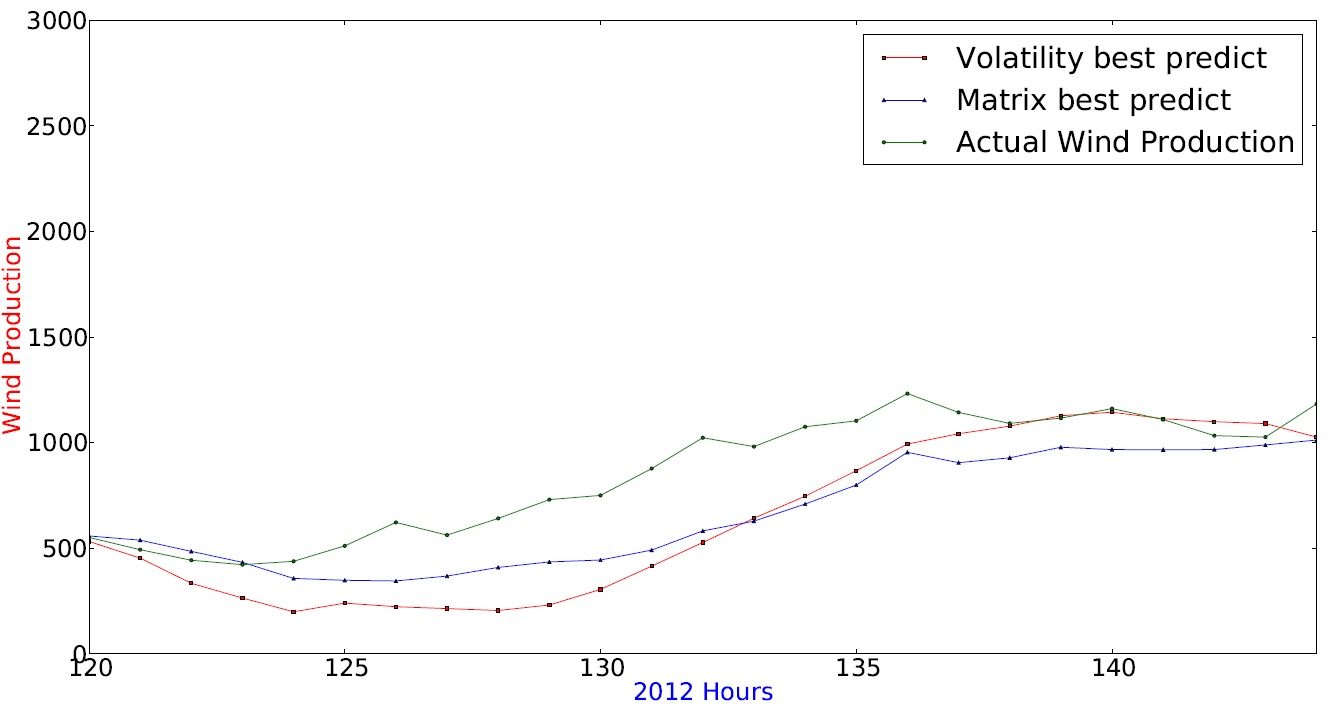
\includegraphics[width=0.99\linewidth]{billeder/bestVolatility120to144.png}
\caption{Wind production prediction for hours 120-144 in 2012 with historical volatility}
\label{fig:bestVolatility120to144}
\end{figure} 

\begin{figure}[H]
\centering
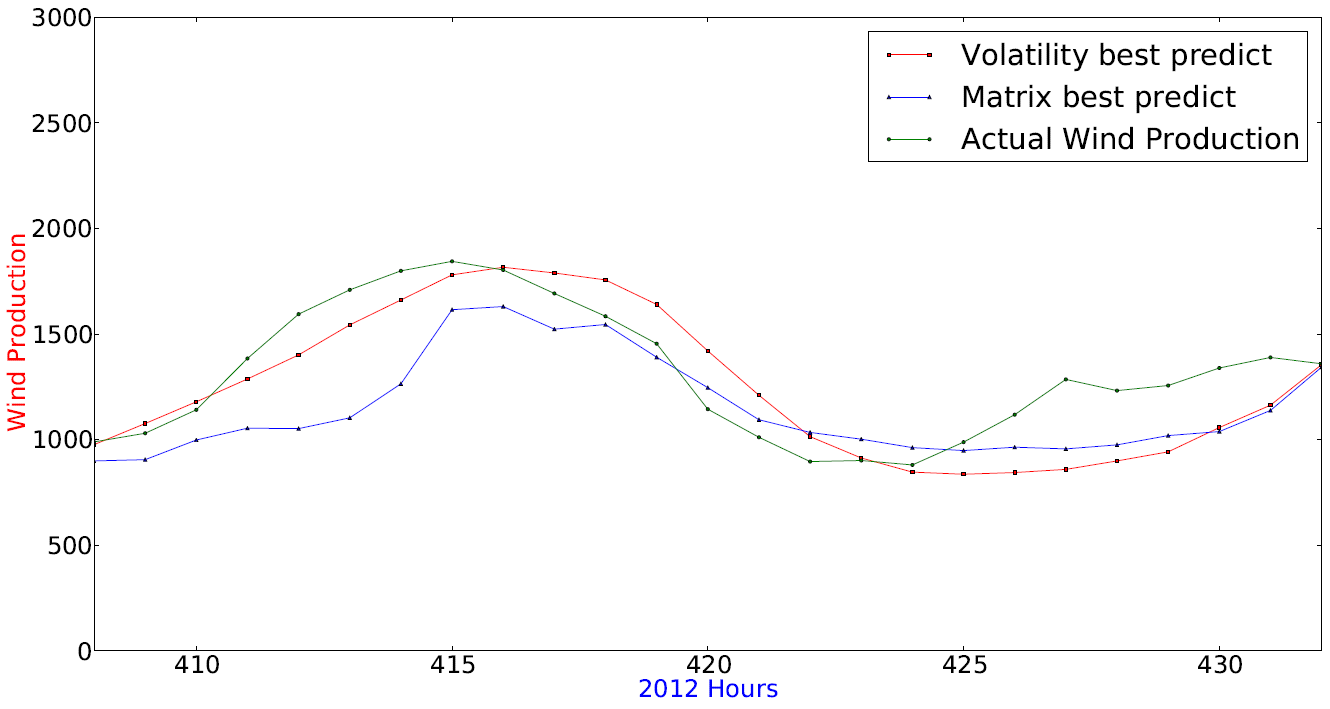
\includegraphics[width=0.99\linewidth]{billeder/bestVolatility408to432.png}
\caption{Wind production prediction for hours 408-432 in 2012 with historical volatility}
\label{fig:bestVolatility408to432}
\end{figure} 

\subsubsection{Conclusion}
Various calculated inputs have been used as input in an attempt to augment the existing generalization based on the meteorological factors. 

\begin{enumerate}
\item Historical volatility by itself showed to be the best calculated input approach with a smoothing factor of 0,70 based on 6 previous hours. The prediction curve moved more rapidly than without any calculated inputs and showed to be better in the higher numbers than low which is what contributes to the overall decrease in MAE. Trade-offs must be made in relation to the specific task but in this thesis the decrease in MAE when using historical volatility will be considered an improvement. The overall improvement in relation to the corresponding combination without it from Table~\ref{table:theWindProdInputParamsTop10WithMatrix} was 3,52\%.
\item The use of scatter and curve resulted in a worsening in MAE. Curve as input was analysed in some detail and the most obvious problem was related to the 24-step-ahead forecasting. When left before a situation very different from what has been seen lately in the training set the curve approach showed difficulties, e.g. trying to predict from the edge of a very steep slope resulted in the curve input pulling the generalization up because a steep slope in general in the training set results in a rising curve. Skewness showed similar results to prediction without any calculated inputs and was therefore not further analysed.
\item It was expected that the statistical approaches in combination could augment each other because they specialize in different areas. This was proven wrong and the results got significantly worse than the best without any calculated inputs. The calculated features are given to high priority when combined and since it cannot be controlled where to predict from it can cause problems when for instance left to predict from the edge of a curve. 
\end{enumerate}

\newpage

\subsection{Experiment Four: Black Box Optimization}
The purpose of experiment four is to find the best number of epochs and dataset size for training. Black box optimization is a way of fine-tuning the network to obtain the best possible prediction.

\subsubsection{Hypothesis}
The size of the training set and number of epochs influence the prediction and from that assume the following:
\begin{enumerate}
\item It is the assumption that too many epochs will result in an over-fitting over the network and therefore a worse prediction. Too few epochs will be under-fit and also a bad prediction.
\item It is expected that a too big or small dataset will result in worse predictions. Too little data will be hard to generalize upon and too much data can bring too much noise.
\end{enumerate}

\subsubsection{Variables}
The best combination of variables has been concluded from previous experiments and will be the basis for the black box optimization. 

\begin{itemize}
\item Wind speed (WS).
\item Time of day as matrix (ToD).
\item Temperature (T).
\item Last known production (L-P).
\item Historical volatility with 0,70 on 6 previous hours (V).
\end{itemize}

The parameters are tested with the following configurations:

\begin{itemize}
\item Selected values between 1 to 2800 epochs.
\item Training set sizes of 1, 3, 6, 9 and 12 months.
\end{itemize}

\subsubsection{Prediction - Epochs}
The number of epochs influence the prediction significantly which is established in Table~\ref{table:bestPredictionEpochExperiment}. It is obvious that too few epochs will result in the network being "under-trained". It can be seen from 1 and 10 epochs that the initial random weights of the network has not yet been adjusted to reflect the training set and therefore predicts randomly. Furthermore, when the number of epochs reach above 2000 it achieves a worse MAE in general. The best result is obtained by 2-300 epochs but with 1200 right after. The results reflect how different epochs affect the production but also how the network can be under-trained or over-trained by either too many or too few epochs. It is obvious from the table that the time in seconds moves up with the number of epochs. Furthermore, the correct direction percentage has been stable in all of the experiments around 70\% but here it can be seen that training to few epochs will result in the percentage dropping significantly together with the worsening in MAE.


\begin{center}
\begin{longtable}{|c|c|c|c|c|c|}
\hline
\textbf{Epochs} & \textbf{MAPE} & \textbf{MAE} & \textbf{\% Rank} & \textbf{Time (s)} & \textbf{\% Correct Direction} \\
\hline
\endfirsthead
\multicolumn{6}{c}%
{\tablename\ \thetable\ -- \textit{Continued from previous page}} \\
\hline
\textbf{Epochs} & \textbf{MAPE} & \textbf{MAE} & \textbf{\% Rank} & \textbf{Time (s)} & \textbf{\% Correct Direction} \\
\hline
\endhead
\hline \multicolumn{6}{r}{\textit{Continued on next page}} \\
\endfoot
\hline
\endlastfoot
\arrayrulecolor{light-gray}
300 & 18,16\% & 121,02 & 0,0\% & 813 & 73,0\% \\ \hline
200 & 18,28\% & 121,81 & 0,65\% & 631 & 73,0\% \\ \hline
1200 & 18,37\% & 122,43 & 1,17\% & 1650 & 71,0\% \\ \hline
1400 & 18,85\% & 125,63 & 3,81\% & 1720 & 72,0\% \\ \hline
400 & 18,9\% & 125,96 & 4,08\% & 1208 & 70,0\% \\ \hline
1100 & 18,95\% & 126,31 & 4,37\% & 1739 & 71,0\% \\ \hline
600 & 19,09\% & 127,23 & 5,13\% & 1483 & 70,0\% \\ \hline
50 & 19,34\% & 128,89 & 6,5\% & 580 & 70,0\% \\ \hline
1500 & 20,2\% & 134,61 & 11,23\% & 2381 & 69,0\% \\ \hline
1300 & 20,68\% & 137,84 & 13,9\% & 1981 & 68,0\% \\ \hline
700 & 20,92\% & 139,45 & 15,23\% & 1152 & 73,0\% \\ \hline
1600 & 21,0\% & 139,95 & 15,64\% & 1720 & 72,0\% \\ \hline
800 & 21,05\% & 140,32 & 15,95\% & 966 & 72,0\% \\ \hline
500 & 21,08\% & 140,49 & 16,09\% & 913 & 72,0\% \\ \hline
150 & 21,18\% & 141,15 & 16,63\% & 669 & 72,0\% \\ \hline
900 & 21,36\% & 142,34 & 17,62\% & 972 & 72,0\% \\ \hline
2200 & 21,47\% & 143,1 & 18,24\% & 1812 & 72,0\% \\ \hline
2600 & 21,52\% & 143,46 & 18,54\% & 3159 & 72,0\% \\ \hline
1800 & 21,58\% & 143,82 & 18,84\% & 2085 & 72,0\% \\ \hline
2400 & 21,59\% & 143,88 & 18,89\% & 2105 & 72,0\% \\ \hline
1000 & 21,78\% & 145,14 & 19,93\% & 1101 & 71,0\% \\ \hline
40 & 22,24\% & 148,21 & 22,47\% & 437 & 71,0\% \\ \hline
2800 & 22,98\% & 153,19 & 26,58\% & 3159 & 72,0\% \\ \hline
2000 & 23,2\% & 154,6 & 27,75\% & 2045 & 71,0\% \\ \hline
20 & 24,0\% & 159,98 & 32,19\% & 441 & 66,0\% \\ \hline
10 & 96,73\% & 644,72 & 432,74\% & 423 & 45,0\% \\ \hline
1 & 149,64\% & 997,34 & 724,11\% & 464 & 50,0\% \\ \hline
\caption{Best prediction with different epochs on same network (H1: 3 and H2: 17)}
\label{table:bestPredictionEpochExperiment}
\end{longtable}
\end{center}

\subsubsection{Prediction - Dataset size}
The size of the dataset has already been discussed during the initial experiments with the best combination of input parameters. Too large training sets can result in over-training as described in\cite{1}, e.g. the dataset contains a lot of different cases and because of that has difficulties when predicting the unseen data of only 24 hours. The over-training consists in the network generalizing upon all cases which can become noise when trying to predict only one of these cases. This corresponds well with wind power production and its high volatility and seasonal. This must be differentiated with over-fitting with too many epochs where weights are being adjusted to the same training set over and over again whereas it in the case of data size simply "knows to much" because too much data makes it hard to generalize. Over-fitting is described in Section~\ref{sec:annSection}. If a training set contains many of the same cases the over-training will be much similar to the one with epochs since it will see the same case over and over again. The weights will be adjusted to that same case again and again and a lower number of epochs are needed. The training set must not be too small because it needs enough cases to generalize upon. Different training set sizes have been tried and the results can be seen in Table~\ref{table:bestPredictionDatasetSizeTest}. The result is as expected since both the small and big datasets are outperformed by the 3 month --- the best have been run again and the new result is much equal to what we saw before. Furthermore, time increases with the size of the data and the 2nd lowest is the best prediction.

\begin{center}
\begin{longtable}{|c|c|c|c|c|c|}
\hline
\textbf{Size} & \textbf{MAPE} & \textbf{MAE} & \textbf{\% Deviation} & \textbf{Time (s)} & \textbf{\% Correctio Direction} \\
\hline
\endfirsthead
\multicolumn{6}{c}%
{\tablename\ \thetable\ -- \textit{Continued from previous page}} \\
\hline
\textbf{Size} & \textbf{MAPE} & \textbf{MAE} & \textbf{\% Deviation} & \textbf{Time (s)} & \textbf{\% Correctio Direction} \\
\hline
\endhead
\hline \multicolumn{6}{r}{\textit{Continued on next page}} \\
\endfoot
\hline
\endlastfoot
\arrayrulecolor{light-gray}
 2200 & 18,4\% & 122,65 & 0,0\% & 631 & 72\% \\ \hline
 8600 & 22,03\% & 146,83 & 19,7\% & 1585 & 72\% \\ \hline
 4200 & 23,56\% & 157,01 & 28,01\% & 855 & 71\% \\ \hline
 1000 & 24,72\% & 164,73 & 34,31\% & 462 & 70\% \\ \hline
 6600 & 26,46\% & 182,31 & 48,64\% & 908 & 70\% \\ \hline
\caption{Best prediction with different training set sizes}
\label{table:bestPredictionDatasetSizeTest}
\end{longtable}
\end{center}

\subsubsection{Hidden Layers and Neurons}
Done by pruning. Is it necessary to say something about the network size or can we rely on the literature telling us that pruning is a tool to find the best network?

\subsubsection{Prediction Graphs}
\label{sec:windPowerBestPredictionGraphs}
The best prediction obtains a MAE of 121 with 300 epochs. Due to the random initialization of weights in the Artificial Neural Network the prediction will vary from time to time. Table~\ref{table:bestPredictionDatasetSizeTest} show how the best prediction changed to 122,65 but still fairly close to 121,02. The experimental results are not 100\% definitive but they have shown tendencies in what works and what does not. A whole year (as used here) contains the different seasonal impacts but at the same time many similar days so that the same situations are predicted more than once. The figures~\ref{fig:bestWPPredictWinter}, ~\ref{fig:bestWPPredictSpring}, ~\ref{fig:bestPredictWPSummer} and ~\ref{fig:bestPredictWPFall} show examples of the behaviour in different seasons and how the prediction is able to handle them. One thing that is noticeable is during fall during the falling curve in 7150-7250 but this is expected due to the high volatility (as mentioned in Section~\ref{sec:bestInputCombiGraph} significant volatility makes it harder to predict). The graphs also shows the need for predicting a whole year due to the obvious differences in the wind power behaviour but at the same time illustrate the predictions ability to follow the development of the ideal wind power. We consider it satisfactory according the the purpose of being able to approach the wind power and at the same time identifying wind power influential factors in the Danish electricity market. Furthermore, an improvement in accuracy has been seen throughout the experiments.

\begin{figure}[H]
\centering
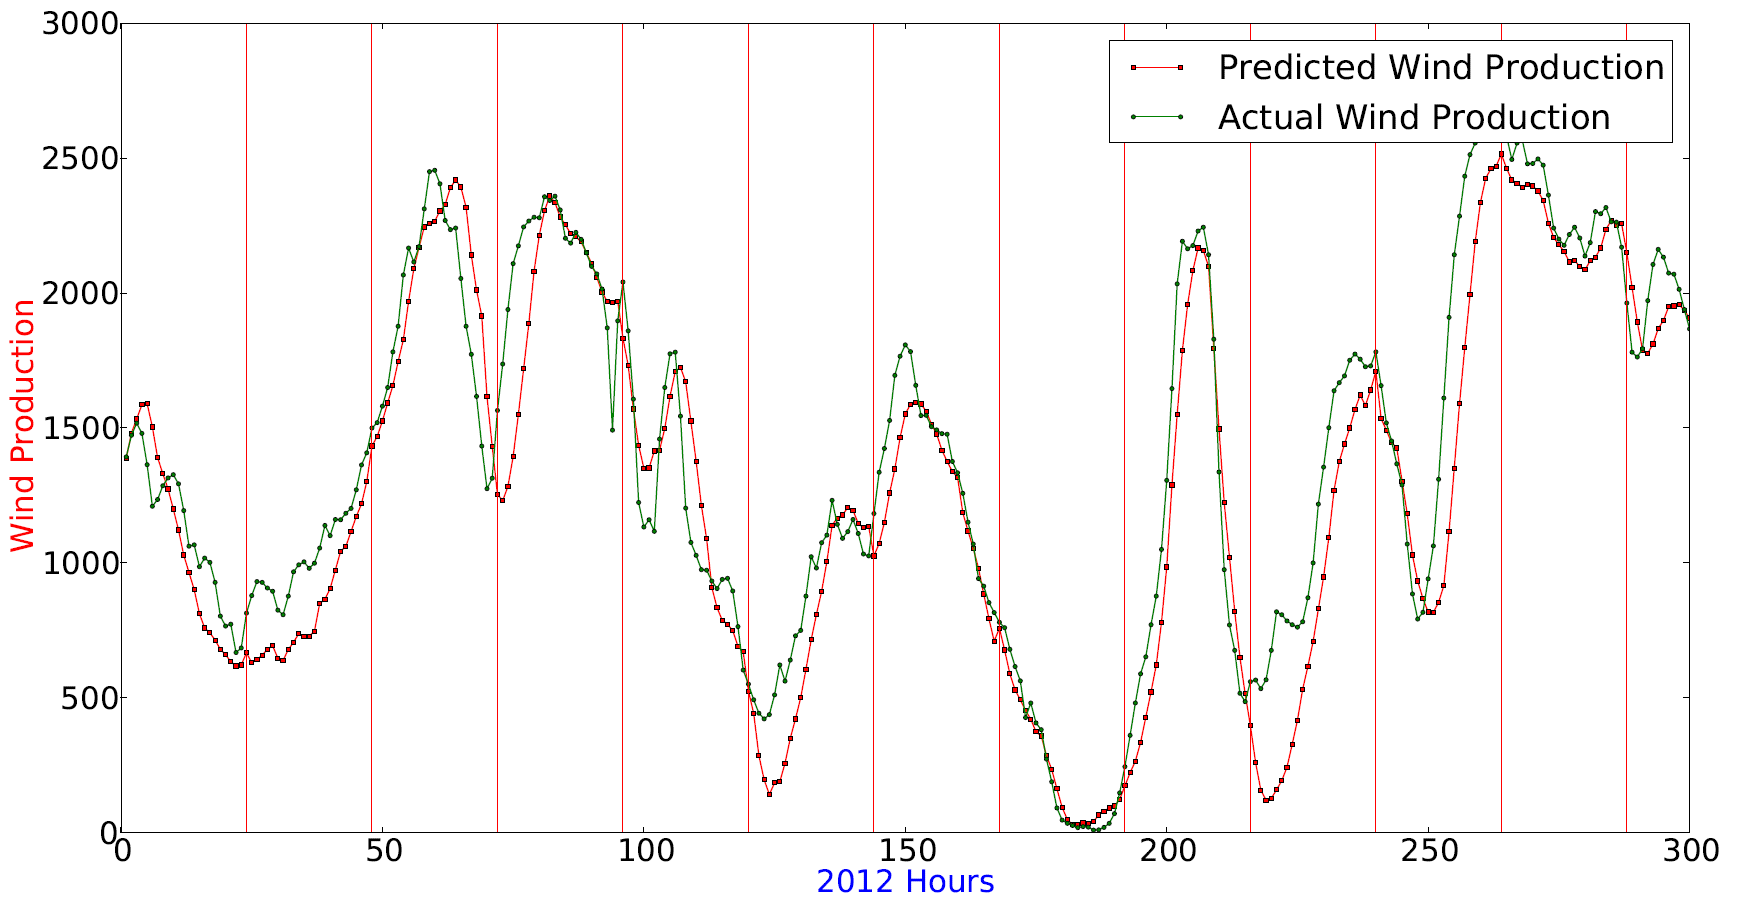
\includegraphics[width=0.99\linewidth]{billeder/bestPossiblePredictionWindProduction0-300.png}
\caption{Best prediction for 300 hours of January (Winter)}
\label{fig:bestWPPredictWinter}
\end{figure}

\begin{figure}[H]
\centering
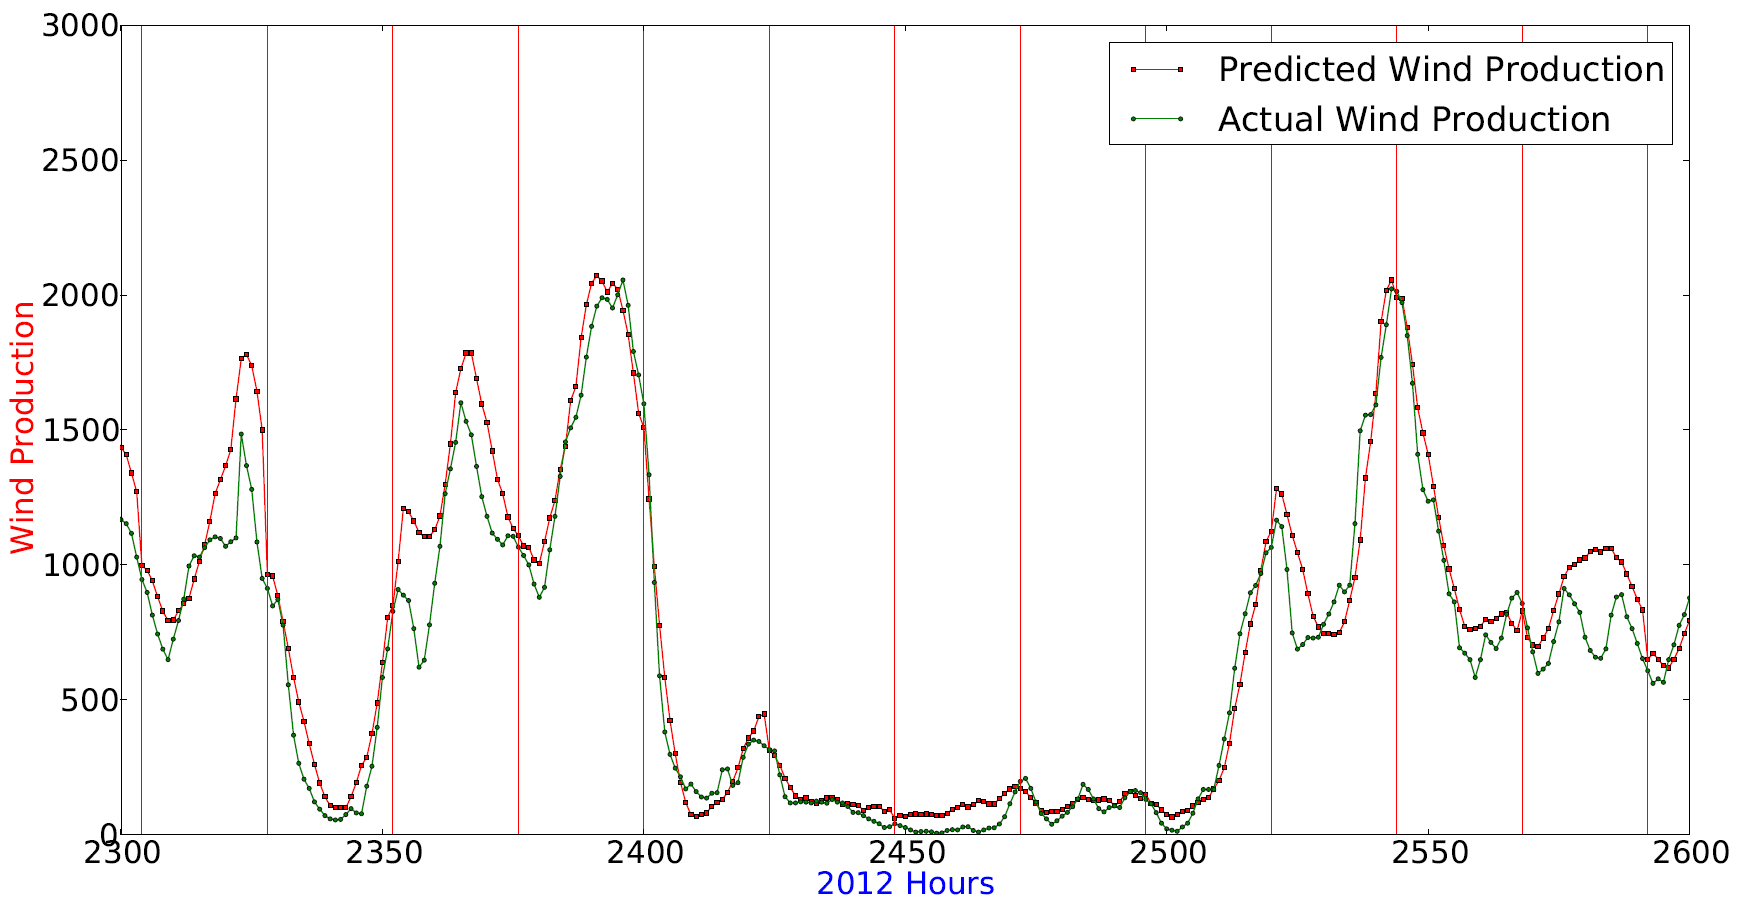
\includegraphics[width=0.99\linewidth]{billeder/bestPossiblePredictionWindProduction2300-2600_April_Spring.png}
\caption{Best prediction for 300 hours of April (Spring)}
\label{fig:bestWPPredictSpring}
\end{figure}

\begin{figure}[H]
\centering
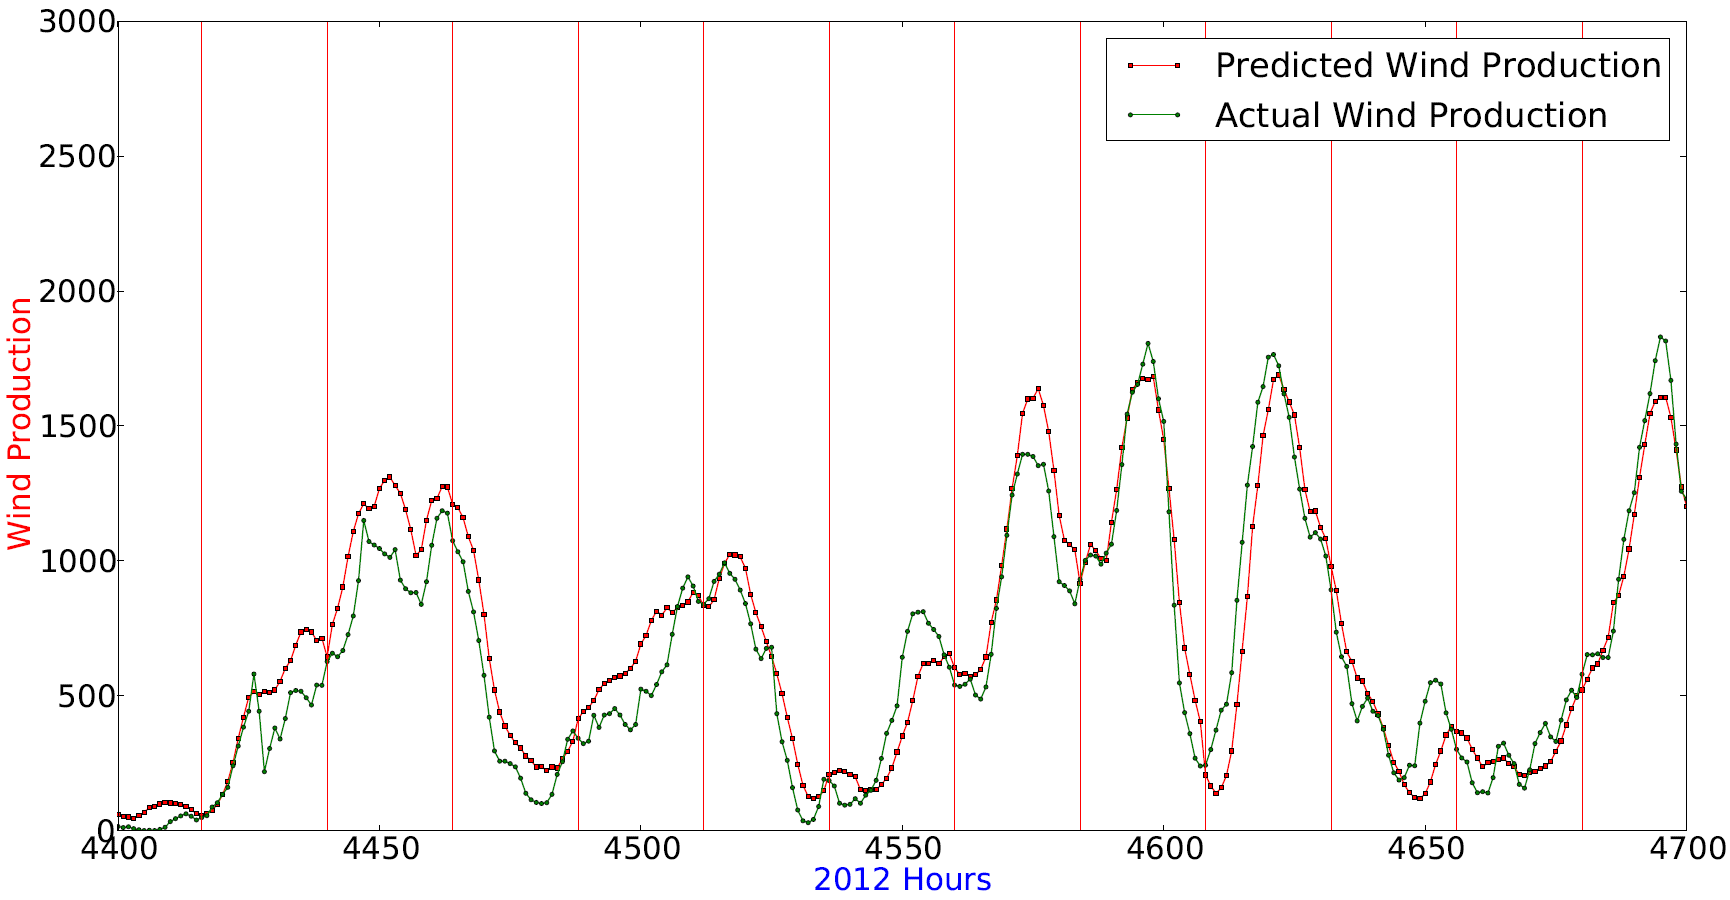
\includegraphics[width=0.99\linewidth]{billeder/bestPossiblePredictionWindProduction4400-4700-Summer.png}
\caption{Best prediction for 300 hours of July (Summer)}
\label{fig:bestPredictWPSummer}
\end{figure}

\begin{figure}[H]
\centering
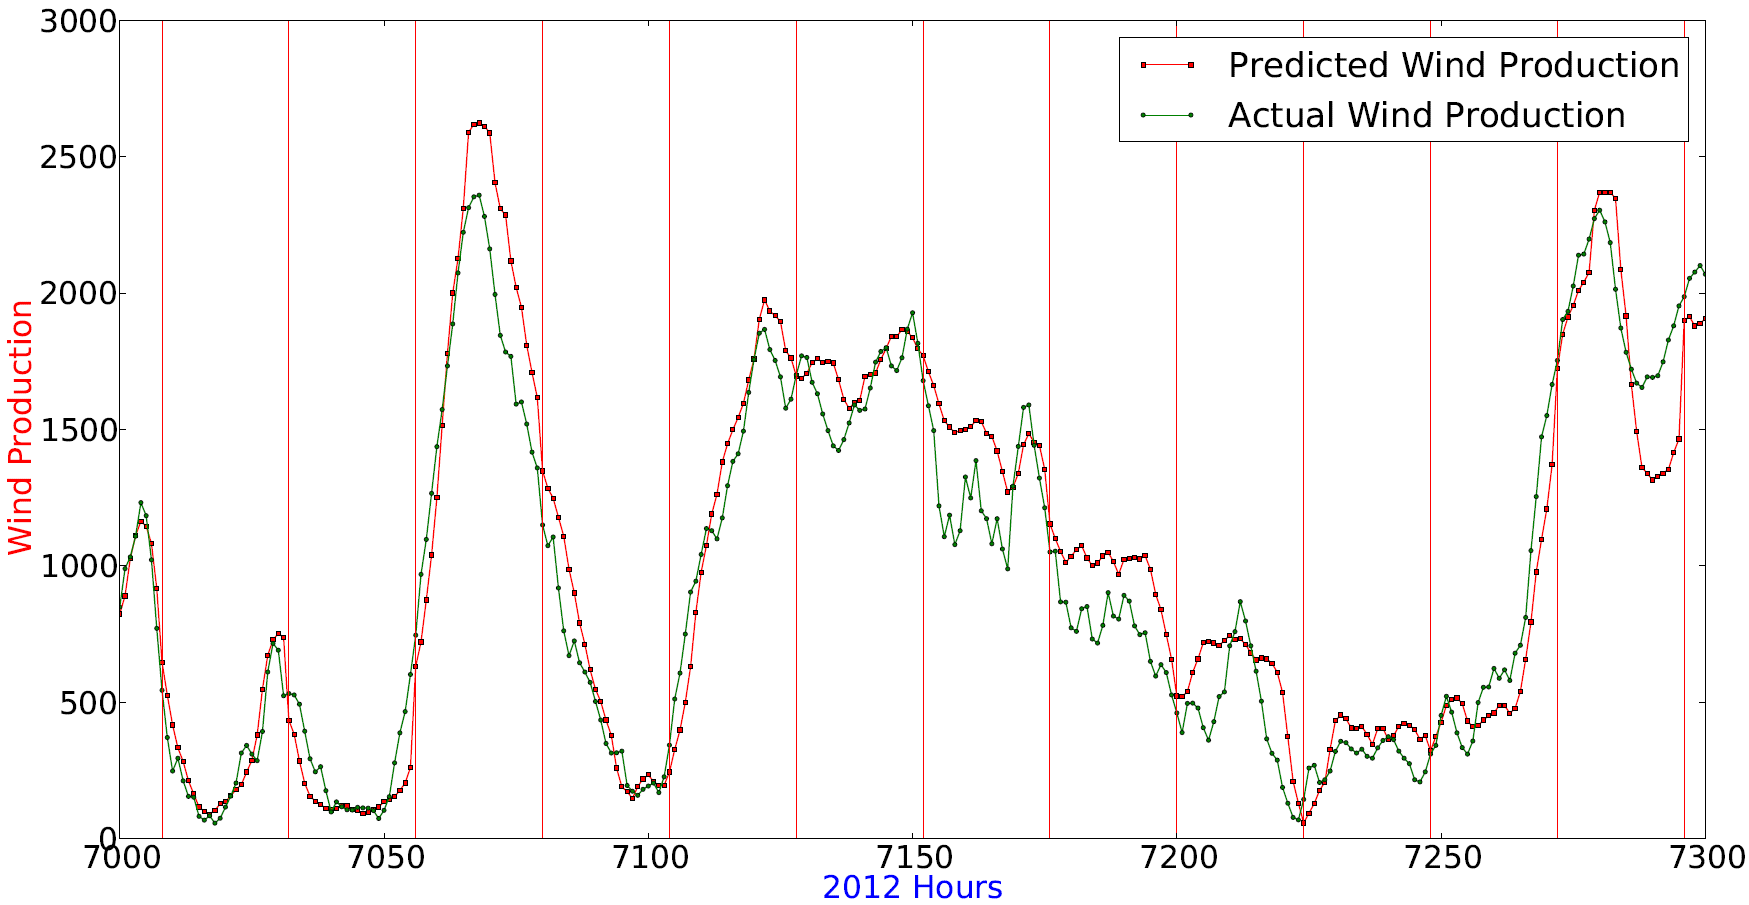
\includegraphics[width=0.99\linewidth]{billeder/bestPossiblePredictionWindProduction7000-7300_Fall.png}
\caption{Best prediction for 300 hours for Oct-Nov (Fall)}
\label{fig:bestPredictWPFall}
\end{figure}

\subsubsection{Conclusion}
Different training set sizes and epochs have been tested and used for prediction.

\begin{enumerate}
\item The results clearly showed the effects of different number of epochs. The expectation was to see under-training and over-training with too many and too few epochs which was confirmed. The best number was 2-300 epochs and the worst 2800, 2000, 20, 10 and 1.
\item Different size of the training set was expected to influence the prediction heavily which was also based on earlier experiences in the first experiments. This was confirmed by the results which showed the best to be on 3 month and the worst to be 3/4 of a year.
\item The predictions graphs presented for the best prediction clearly showed the ability of following the behaviour of the ideal wind power and an improvement in mae in relation to the first experiment. 
\end{enumerate}

\subsection{Experiment Five - Step-ahead forecasting}
\label{sec:windPowerExperimentFive}
The purpose is to identify the error in different step-ahead forecasts from 1 hour to 24 hour. In step-ahead forecasting every step is dependent on the prediction from the step just before it but for wind power production that does not necessarily mean that many steps will be the worst since it follows wind speed significantly which will make it possible to correct during the prediction.

\subsubsection{Hypothesis}
It is expected to see an improved error when very few steps is included in the step-ahead forecasting. When the number of steps reach a certain point the results is expected to become more random.

\subsubsection{Prediction}
Table~\ref{table:stepAheadForecastingWindProduction} shows the results from the step-ahead testing. It is clear that low numbers until 9 is significantly better than the rest. The expectation was to see a more random distribution when reaching a certain point but there is a clear tendency in the high numbers in the button and low numbers in the top. The obvious problem with the results is that they are all predicting the same year and therefore predicting from different places in relation to the number of steps. It will results in the results being incomparable since the prediction starting point is not the same which heavily affects the predictions as discussed in Section~\ref{sec:combiningTheApproachesWP}. This problem becomes more clear when looking at Figure~\ref{fig:best22vsbest24Ahead} where it is obvious that 22-step-ahead starts much differently than 24-step-ahead in Figure~\ref{best24AheadPredictionWithLines}. It has huge effect on the prediction which would also apply in a real life setting. It could again be a discussion about reconfigurability of the ann when used in a decision making setting. The experience of the user comes into place in these predictions because it greatly influences the result where to start from. This is further backed up by Table~\ref{table:stepAheadForecastingWindProduction}.

\begin{center}
\begin{longtable}{|c|c|c|c|c|}
\hline
\textbf{Steps ahead} & \textbf{MAPE} & \textbf{MAE} & \textbf{\% Deviation} & \textbf{\% Correct Direction}  \\
\hline
\endfirsthead
\multicolumn{5}{c}%
{\tablename\ \thetable\ -- \textit{Continued from previous page}} \\
\hline
\textbf{Steps ahead} & \textbf{MAPE} & \textbf{MAE} & \textbf{\% Deviation} & \textbf{\% Correct Direction}  \\
\hline
\endhead
\hline \multicolumn{5}{r}{\textit{Continued on next page}} \\
\endfoot
\hline
\endlastfoot
\arrayrulecolor{light-gray}
1 & 7,7\% & 51,5 & 0,0\% & 74\%  \\ \hline
2 & 9,85\% & 65,91 & 27,98\% & 70\%  \\ \hline
3 & 11,8\% & 78,94 & 53,28\% & 71\%  \\ \hline
4 & 13,73\% & 91,87 & 78,39\% & 70\%  \\ \hline
6 & 15,05\% & 100,66 & 95,46\% & 70\%  \\ \hline
5 & 15,48\% & 103,58 & 101,13\% & 70\%  \\ \hline
9 & 16,51\% & 110,47 & 114,5\% & 72\%  \\ \hline
7 & 16,52\% & 110,53 & 114,62\% & 72\%  \\ \hline
11 & 17,47\% & 116,88 & 126,95\% & 70\%  \\ \hline
8 & 18,18\% & 121,62 & 136,16\% & 68\%  \\ \hline
24 & 18,38\% & 122,51 & 137,88\% & 73\%  \\ \hline
17 & 18,89\% & 125,87 & 144,41\% & 69\%  \\ \hline
19 & 19,5\% & 129,88 & 152,19\% & 69\%  \\ \hline
23 & 19,56\% & 130,85 & 154,08\% & 72\%  \\ \hline
15 & 19,89\% & 132,94 & 158,14\% & 72\%  \\ \hline
16 & 20,16\% & 134,37 & 160,91\% & 72\%  \\ \hline
10 & 20,1\% & 134,5 & 161,17\% & 73\%  \\ \hline
14 & 20,42\% & 136,6 & 165,24\% & 67\%  \\ \hline
12 & 20,49\% & 137,09 & 166,19\% & 67\%  \\ \hline
20 & 20,69\% & 137,79 & 167,55\% & 73\%  \\ \hline
13 & 20,64\% & 138,11 & 168,17\% & 72\%  \\ \hline
18 & 20,79\% & 138,97 & 169,84\% & 72\%  \\ \hline
21 & 21,05\% & 140,8 & 173,4\% & 68\% \\ \hline
22 & 21,87\% & 146,28 & 184,04\% 66\% \\ \hline
\caption{Step-ahead prediction from 1-24}
\label{table:stepAheadForecastingWindProduction}
\end{longtable}
\end{center}

All starting positions have been tried in Table~\ref{table:stepAheadForecastingWindProductionStartingPositions} and it supports what was concluded from Table~\ref{table:stepAheadForecastingWindProduction}. The position that has always been used is marked with an x. It is obvious here that the exact same prediction applied at various starting points differs much in accuracy. 

\begin{center}
\begin{longtable}{|c|c|c|c|c|}
\hline
\textbf{Steps ahead} & \textbf{MAPE} & \textbf{MAE} & \textbf{\% Deviation} & \textbf{\% Correct Direction} \\
\hline
\endfirsthead
\multicolumn{5}{c}%
{\tablename\ \thetable\ -- \textit{Continued from previous page}} \\
\hline
\textbf{Steps ahead} & \textbf{MAPE} & \textbf{MAE} & \textbf{\% Deviation} & \textbf{\% Correct Direction} \\
\hline
\endhead
\hline \multicolumn{5}{r}{\textit{Continued on next page}} \\
\endfoot
\hline
\endlastfoot
\arrayrulecolor{light-gray}
16 & 18,26\% & 121,73 & 0,0\% & 73\%  \\ \hline
1 (x) & 18,49\% & 123,25 & 1,25\% & 73\%  \\ \hline
8 & 18,61\% & 124,06 & 1,91\% & 72\%  \\ \hline
7 & 18,68\% & 124,52 & 2,29\% & 70\%  \\ \hline
14 & 18,92 & 126,12 & 3,67\% & 70\%  \\ \hline
13 & 19,12\% & 127,49 & 4,73\% & 70\%  \\ \hline
22 & 19,5\% & 129,94 & 6,74\% & 69\%  \\ \hline
17 & 19,58\% & 130,49 & 7,2\% & 70\%  \\ \hline
5 & 20,94\% & 139,56 & 14,65\% & 72\%  \\ \hline
24 & 20,97\% & 139,79 & 14,84\% & 72\%  \\ \hline
12 & 21,03\% & 140,15 & 15,13\% & 72\%  \\ \hline
3 & 21,04\% & 140,23 & 15,2\% & 72\%  \\ \hline
2 & 21,09\% & 140,57 & 15,48\% & 72\%  \\ \hline
19 & 21,1\% & 140,62 & 15,52\% & 72\%  \\ \hline
20 & 21,11\% & 140,68 & 15,57\% & 72\%  \\ \hline
10 & 21,13\% & 140,85 & 15,71\% & 72\%  \\ \hline
21 & 21,18\% & 141,19 & 15,99\% & 72\%  \\ \hline
18 & 21,19\% & 141,2 & 15,99\% & 72\%  \\ \hline
4 & 21,23\% & 141,51 & 16,25\% & 72\%  \\ \hline
23 & 21,31\% & 142,01 & 16,66\% & 72\%  \\ \hline
15 & 21,47\% & 143,08 & 17,54\% & 72\%  \\ \hline
11 & 21,57\% & 143,74 & 18,08\% & 72\%  \\ \hline
6 & 21,61\% & 144,04 & 18,33\% & 72\%  \\ \hline
9 & 22,71\% & 151,36 & 24,34\% & 71\%  \\ \hline
\caption{24-step-aheads forecast covering all starting positions}
\label{table:stepAheadForecastingWindProductionStartingPositions}
\end{longtable}
\end{center}

\begin{figure}[H]
\centering
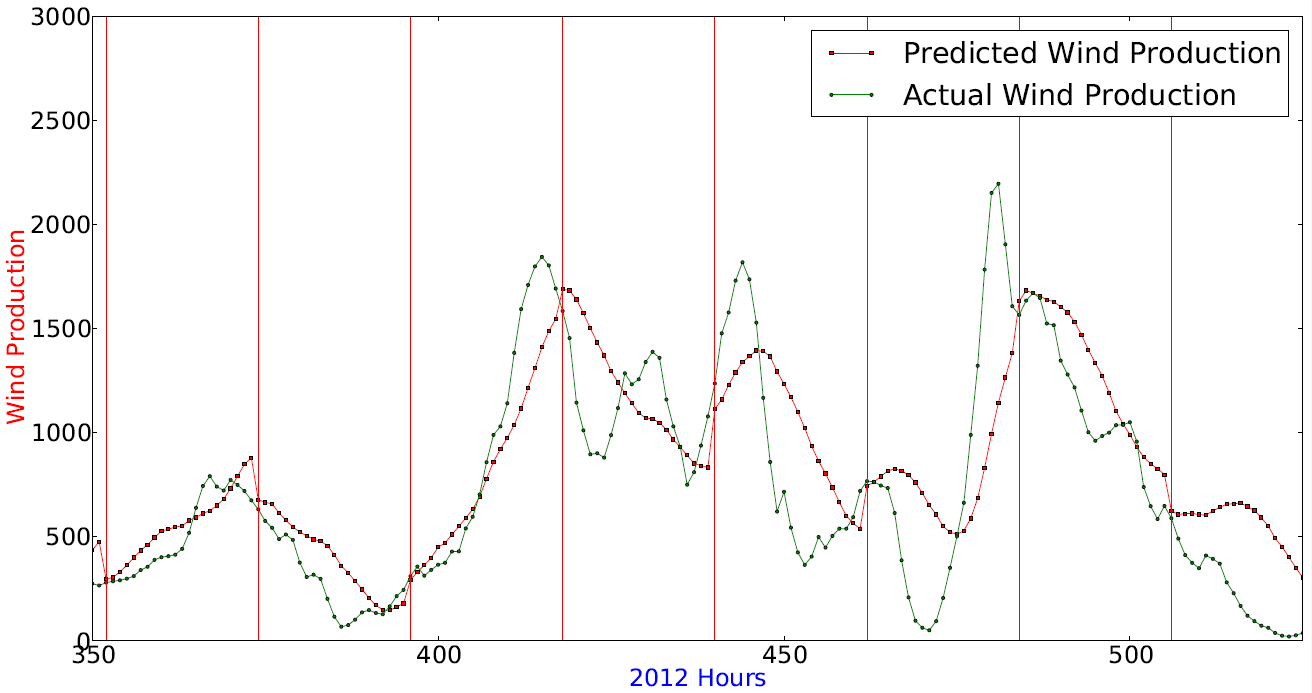
\includegraphics[width=0.99\linewidth]{billeder/best22vsbest24Ahead.png}
\caption{22-step-ahead forecast}
\label{fig:best22vsbest24Ahead}
\end{figure}

\begin{figure}[H]
\centering
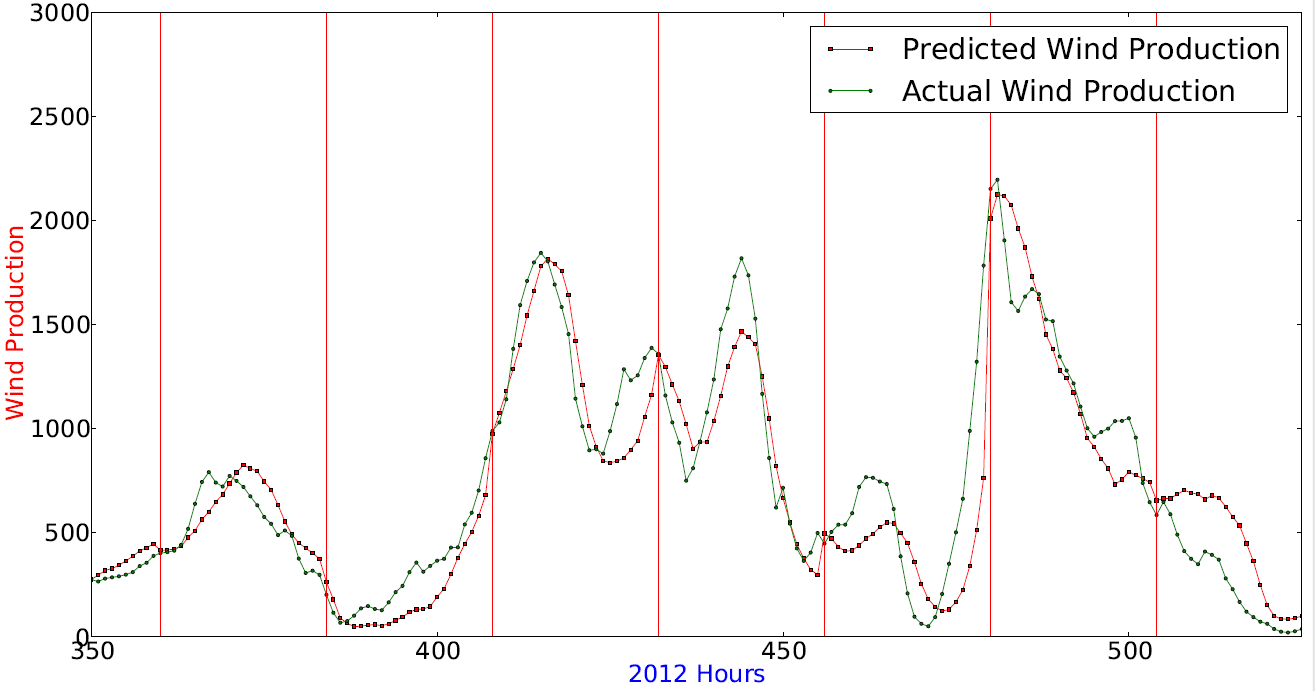
\includegraphics[width=0.99\linewidth]{billeder/best24AheadPredictionWithLines.png}
\caption{24-step-ahead forecast}
\label{fig:best24AheadPredictionWithLines}
\end{figure} 

\todo{one step ahead vs. 24 ahead to show that is the same in the beginning on 24 timer}

\subsubsection{Conclusion}
The expectation was to see an improvement in MAE when predicting fewer hours which was seen in Table~\ref{table:stepAheadForecastingWindProduction}. It also showed that at some point the fewer hours is not necessarily better because they start at different positions and the prediction can correct itself the further it gets. The starting position has a huge impact on the accuracy of the prediction which was illustrated in the comparison between 22- and 24-step-ahead forecasts. It was further backed up by trying out all starting points with 24-step-ahead forecasting.

\subsection{Concluding Remarks}
Experiments have been conducted to identify the best combination of inputs as well as the impact of data manipulation, calculated inputs and black box optimization. Each experiment concludes on its findings in relation to experiments before it and expectations from the wind power production analysis. Table~\ref{table:comparisonOfResultsWindProduction} shows the overall improvement of 5,35\% from the first experiment to the last. Experiment five is left out in this table because it cannot be compared with the other since it predicts different number of hours. What have been observed throughout all experiments is the stable percentage of around 70\% in predicting the correct direction. It has also been discussed that the stability here lies in the co-relation to wind speed which is included as input in all experiments. The best result missed its target (in average) by 121 out of the interval from 0 to 2753 corresponding to 4,4\% of the 2753 potential values. We consider this to be satisfactory since it gives a clear indication of the wind power movements which was the purpose of the wind power prediction according to Section~\ref{sec:windPowerAnalysis}. 

\begin{enumerate}
\item First experiment showed the importance of the correct input parameters used in the Artificial Neural Network. Temperature, last known production, wind speed and time of day was the best combination. Air density and wind direction also showed themselves in top-3. Furthermore, too large datasets seriously decreased the accuracy due to over-training of the network.
\item Experiment two showed a slight increase (1,9\% in average improve for top-3) in accuracy when applying matrix on time of day. Trimming makes less sense in a prediction simulation for Wind Power since no completely irregular values exist in the wind power training set. The predictions with trimming showed a decrease in accuracy compared to without trimming because trimming ended up creating irregularities instead of removing them.
\item Third experiment tried different approaches to calculated inputs in relation to letting the network itself calculate statistics by adding various previous productions --- the approaches are slope calculation, skewness and volatility. The best of the approaches were volatility which obtained an increase of 3,52\% in relation to the prediction just without it.
\item The purpose of the fourth experiment was to identify the correct number of epochs and validate the correct size of the training set. The best size was 3 month of data and with 2-300 epochs. The experiment also illustrated how the network can easily be under- or overfitted with too many or few epochs, or be under- or overtrained  according to the size of the training set. The best prediction is considered to be in agreement with our purpose, namely to approach the wind power by applying different strategies and identifying what works and what does not.	
\item The fifth experiment regarding step-ahead forecasting illustrated how the error can be elevated due to how subsequent steps depend on the prediction from its predecessor. This experiment also uncovered the huge difference in starting points of the prediction. The results varied all the way from 121,73 to 151,36 in MAE. The best best configuration of input parameters, epochs and size of data is still considered to be the best since all experiments had the same starting point and therefore predicted the same hours in all steps. This will be discussed further.
\end{enumerate}

\footnotesize
\begin{center}
\begin{longtable}{|c|c|c|c|c|}
\hline
\textbf{Exp: 1} & \textbf{Exp: 2} & \textbf{Exp: 3} & \textbf{Exp: 4} & \textbf{Overall improvement} \\
\hline
\endfirsthead
\multicolumn{5}{c}%
{\tablename\ \thetable\ -- \textit{Continued from previous page}} \\
\hline
\textbf{Exp: 1} & \textbf{Exp: 2} & \textbf{Exp: 3} & \textbf{Exp: 4} & \textbf{Overall improvement} \\
\hline
\endhead
\hline \multicolumn{5}{r}{\textit{Continued on next page}} \\
\endfoot
\hline
\endlastfoot
\arrayrulecolor{light-gray}
128,32 &  126,25 & 121,81 & 121,02 & 5,7\% \\ \hline
\caption{Comparison of the best MAE from each of the experiment except from the fifth}
\label{table:comparisonOfResultsWindProduction}
\end{longtable}
\end{center}
\normalsize

\footnotesize
\begin{center}
\begin{longtable}{|c|c|c|c|c|}
\hline
\textbf{Exp: 1} & \textbf{Exp: 2} & \textbf{Exp: 3} & \textbf{Exp: 4} & \textbf{Overall improvement} \\
\hline
\endfirsthead
\multicolumn{5}{c}%
{\tablename\ \thetable\ -- \textit{Continued from previous page}} \\
\hline
\textbf{Exp: 1} & \textbf{Exp: 2} & \textbf{Exp: 3} & \textbf{Exp: 4} & \textbf{Overall improvement} \\
\hline
\endhead
\hline \multicolumn{5}{r}{\textit{Continued on next page}} \\
\endfoot
\hline
\endlastfoot
\arrayrulecolor{light-gray}
19,25\% &  18,94\% & 18,28\% & 18,16\% & 1,09\% \\ \hline
\caption{Comparison of the best MAPE from each of the experiment except from the fifth}
\label{table:comparisonOfResultsWindProduction}
\end{longtable}
\end{center}
\normalsize